\documentclass[
  10pt,               % 120% Schriftgrösse
  oneside,            % einsitiger Druck
  a4paper,            % A4
  titlepage,          % inklusive Titelpage
  pointlessnumbers,	  % Kein Punkt hinter der Kapitelnummerierung
  halfparskip,        % Europäischer Satz mit abstand zwischen Absätzen
  pdftex,             % Direkt ins Pdf übersetzen, keine Kapitel
  liststotoc,         % Inhaltsverzeichnis inkl. Abbildungsverzeichnis
  bibtotoc]{scrreprt} % Inhaltsverzeichnis inkl. Literaturverzeichnis

%%%%%%%%%%%%%%%%%%%%%%%%%
% Allgemeine Packete    %
%%%%%%%%%%%%%%%%%%%%%%%%%

% Neue Rechtschreibung
\usepackage[german, ngerman]{babel}

% UTF 8
\usepackage[utf8]{inputenc}
\usepackage{nicefrac}
\usepackage{multirow}

% Ausgabefonts
\usepackage[T1]{fontenc}

% Euro Symbol (\texteuro}
\usepackage{textcomp}

% für die Gesamtseitenzahl
\usepackage{totpages}

% Paket für Farben
\usepackage{color}

% Bilder
%\usepackage{graphicx}

% Fliesstext um Bilder
\usepackage{wrapfig}

% Tabellen mit definierter Breite und zentriert
\usepackage{array}

\newcolumntype{x}[1]{%
>{\centering\hspace{0pt}}p{#1}}%

% Glossar alt
%\usepackage[style=super, header=none, border=none, number=none, cols=2, toc=true]{glossary}
%\makeglossary

% Glossar neu
%\usepackage{glossaries}
%\makeglossaries
%\printglossaries

% mehrere Befehle für die Tabellen
\usepackage{booktabs}

%Packet für absolut Positionierte Textboxen
\usepackage[absolute]{textpos} %showboxes zum besseren positionieren

% Packet für Boxen
%\usepackage{framed}

% Initialen
%\usepackage{lettrine}
%\DeclareFixedFont{\Yinit}{U}{yinit}{m}{n}{16}

% Umbruch von langen Wörtern
\usepackage{seqsplit}


%%%%%%%%%%%%%%%%%%%%%%%%%
% Seiteneinstellungen   %
%%%%%%%%%%%%%%%%%%%%%%%%%
\usepackage[
  portrait,
%   twoside,
  left=40mm,
  top=20mm,
  textwidth=145mm,
  textheight=252mm,
  %head=15mm,
  head=15mm,
  headsep=5mm,
  foot=8mm
]{geometry}

% Text muss nicht umbedingt bis zur Fusszeile reichen
\raggedbottom

%\usepackage[cam,axes,a3,center]{crop}
%\usepackage[frame,a4,center]{crop}

%%%%%%%%%%%%%%%%%%%%%%%%%
% Schriftart            %
%%%%%%%%%%%%%%%%%%%%%%%%%

%\usepackage{courier}  % Courier für Code verwenden
%\usepackage{helvet}   % Helvetica
% Helvetic als Font verwenden
%\renewcommand{\familydefault}{\sfdefault}


%%%%%%%%%%%%%%%%%%%%%%%%%
% Mathematik Packete    %
%%%%%%%%%%%%%%%%%%%%%%%%%

% Verbesserte Mathematik Satz
\usepackage{amsmath}

% Zahlenmenngen in der Mathematik
\usepackage{amssymb}

% Times New Roman für Mathematik
\usepackage{mathptmx}


%%%%%%%%%%%%%%%%%%%%%%%%%
% Inhaltsverzeichnis    %
%%%%%%%%%%%%%%%%%%%%%%%%%
% Punkte im Inhaltsverzeichnis bei Sections
\usepackage{tocloft}
%\renewcommand{\cftsecdotsep}{4.5}
\renewcommand{\cftsecdotsep}{1}
%\setcounter{secnumdepth}{1}
\setcounter{tocdepth}{1}
\setcounter{secnumdepth}{1}

%%%%%%%%%%%%%%%%%%%%%%%%%
% Literaturverzeichnis  %
%%%%%%%%%%%%%%%%%%%%%%%%%

%\usepackage[ngerman,ref]{backref}
%\renewcommand{\backrefpagesname}{Zitiert auf S.}
%renewcommand{\refname}{Quellenverzeichnis}

%%%%%%%%%%%%%%%%%%%%%%%%%
% Anhang			    %
%%%%%%%%%%%%%%%%%%%%%%%%%

\newcommand{\anhang}[1]{
	%\setsection{1}
    \setcounter{page}{1}
	\input{#1}
	\newpage
}

%%%%%%%%%%%%%%%%%%%%%%%%%
% Source Code Packete   %
%%%%%%%%%%%%%%%%%%%%%%%%%

% Codesegmente
\usepackage{listings}
\definecolor{darkblue}{rgb}{0,0,0.6}
\definecolor{darkred}{rgb}{0.6,0,0}
\definecolor{darkgreen}{rgb}{0,0.6,0}
\definecolor{red}{rgb}{0.98,0,0}
\lstloadlanguages{C,C++} % entsprechende Sprachen werden hier schon mal geladen, damit das Übersetzen schneller geht
\definecolor{listinggray}{gray}{0.9}
\definecolor{lbcolor}{rgb}{0.9,0.9,0.9}
\lstset{
	backgroundcolor=\color{lbcolor},
    tabsize=4,    
%   rulecolor=,
    language=[GNU]C++,
        basicstyle=\scriptsize,
        upquote=true,
        aboveskip={1.5\baselineskip},
        columns=fixed,
        showstringspaces=false,
        extendedchars=false,
        breaklines=true,
        prebreak = \raisebox{0ex}[0ex][0ex]{\ensuremath{\hookleftarrow}},
        frame=single,
        numbers=left,
        showtabs=false,
        showspaces=false,
        showstringspaces=false,
        identifierstyle=\ttfamily,
        keywordstyle=\color[rgb]{0,0,1},
        commentstyle=\color[rgb]{0.026,0.112,0.095},
        stringstyle=\color[rgb]{0.627,0.126,0.941},
        numberstyle=\color[rgb]{0.205, 0.142, 0.73},
%        \lstdefinestyle{C++}{language=C++,style=numbers}’.
}
\lstset{
    backgroundcolor=\color{lbcolor},
    tabsize=4,
  language=C++,
  captionpos=b,
  tabsize=3,
  frame=lines,
  numbers=left,
  numberstyle=\tiny,
  numbersep=5pt,
  breaklines=true,
  showstringspaces=false,
  basicstyle=\footnotesize,
%  identifierstyle=\color{magenta},
  keywordstyle=\color[rgb]{0,0,1},
  commentstyle=\color{darkgreen},
  stringstyle=\color{red}
  }




%\lstset{%
%  language=C++%,
%  basicstyle=\footnotesize\ttfamily,
%  commentstyle=\itshape\color{darkgreen},
%  keywordstyle=\bfseries\color{darkblue},
%  stringstyle=\color{darkred},
%  showspaces=false,
%  columns=fixed,
%  numbers=left,
%  frame=none,
%  numberstyle=\tiny,
%  breaklines=true,
%  showstringspaces=false,
%  xleftmargin=1cm,
%  tabsize=2
%}%


%%%%%%%%%%%%%%%%%%%%%%%%%
% Makros                %
%%%%%%%%%%%%%%%%%%%%%%%%%

% Makros
\newcommand{\redbox}[1]
{\vspace*{2mm} \\ \fboxsep5mm \fboxrule0.5mm \fcolorbox{red}{white}{\parbox{1.5cm}{
\includegraphics[width=1cm]{Achtung.pdf}}\parbox{13cm}{\textcolor{black}{#1}
}}\vspace*{2mm}\\}

\newcommand{\redboxtitle}[2]
{\vspace*{2mm} \\ \textcolor{red}{\bfseries #1\smallskip} \\ \fboxsep5mm \fboxrule0.5mm \fcolorbox{red}{white}{\parbox{1.5cm}{
\includegraphics[width=1cm]{Achtung.pdf}}\parbox{13cm}{\textcolor{black}{#2}
}}\vspace*{2mm}\\}

% Fuer die Minipage um eine Tabelle und Abbildung nebeneinander Setzen
\makeatletter
\newcommand{\setcaptype}[1]{\renewcommand{\@captype}{#1}}
\makeatother


%%%%%%%%%%%%%%%%%%%%%%%%%
% Kopf und Fusszeile    %
%%%%%%%%%%%%%%%%%%%%%%%%%
% 7. Kopf und Fusszeilen
\usepackage{totpages}               % Paket für die Gesamtseitenzahl
\usepackage{scrpage2}
\pagestyle{scrheadings}
\renewcommand*{\chapterpagestyle}{scrheadings}
\clearscrheadfoot
%\setkomafont{pagefoot}{\normalfont\sffamily}
\automark[]{chapter}
\ihead{VT1: EEROS Sequencer}
\ohead{\headmark}
\setheadsepline{0.5pt}[\color{HeadBlue}] 
\ifoot{Marcel Gehrig}
\ofoot{\today}
\cfoot{- \thepage{} -}
%\setfootsepline{0.5pt}
%%Kopf- und Fusszeile
\definecolor{HeadBlue}{rgb}{0,0.41,0.71}
\definecolor{FootBlack}{rgb}{0,0,0}
\addtokomafont{pagehead}{\color{HeadBlue}} 
\addtokomafont{pagefoot}{\color{FootBlack}}
%\usepackage{eso-pic}
%\usepackage{scrpage2}
%\usepackage{extramarks}
\usepackage[final]{pdfpages}
%%\pagestyle{scrheadings}
%%\clearscrheadfoot
%% Schriftart auf die Normale Schrift setzen
%%\setkomafont{pagefoot}{\normalfont\sffamily}
%%\automark[]{section} % \leftmark zeigt die aktuelle Section an, \rightmark bleibt leer
%
%%Kopfzeile
%%\ihead{NTB}
%%\ohead{\leftmark}
%%\lehead{\hspace*{1cm}\begin{large}\leftmark\end{large} \AddToShipoutPicture*{%
%%  \AtPageUpperLeft{\put(0,\LenToUnit{-9.4mm}){%
%%    \colorbox{HeadBlue}{\parbox[t][6mm]{1.8cm}{\ }}%
%%    \colorbox{black}{\parbox[t][6mm]{0.1cm}{\ }}}}}}
%%\rohead{\begin{large}\leftmark\end{large}\hspace*{1cm} \AddToShipoutPicture*{%
%%  \AtPageUpperLeft{\put(\LenToUnit{\paperwidth},\LenToUnit{-9.4mm}){\kern-2.3cm%
%%    \colorbox{black}{\parbox[t][6mm]{0.1cm}{\ }}%
%%    \colorbox{HeadBlue}{\parbox[t][6mm]{1.8cm}{\ }}}}}}
%%\rehead{\begin{large}NTB\end{large}}
%%\lohead{\begin{large}NTB\end{large}}
%%\setheadsepline{1.2pt}
%\usepackage{ifthen}
%\newboolean{SectionOnPage}
%\renewcommand{\sectionmark}[1]{\setboolean{SectionOnPage}{true}\markboth{#1}{#1}}
%\newcommand{\headerblackbox}{\colorbox{black}{\parbox[c][6mm]{0.1cm}{\ }}}
%\newcommand{\headerbluebox}[1]{\colorbox{HeadBlue}{\parbox[c][6mm]{1.8cm}{%
%%       \ifnum\value{section}>0
%%         \ifthenelse{true}{H}{#1\textbf{\begin{large}\color{white}{\sffamily{\arabic{section}}}\end{large}}}
%%       \else
%          #1 \textbf{\begin{large}\color{white}{\sffamily{\ }}\end{large}}
%%       \fi
%}}}
%\newcommand{\headerbluetext}[1]{\textbf{\begin{large}\color{HeadBlue}{#1}\end{large}}}
%%\newcommand{\headerNTB}{\headerbluetext{NTB}}
%\newcommand{\headerNTB}{\includegraphics[height=1.2cm]{ntb}}
%\newcommand{\headerleftmark}{\headerbluetext{\firstleftmark}}
%
%\lehead{\hspace*{5mm}\headerleftmark \AddToShipoutPicture*{%
%  \AtPageUpperLeft{\put(0,\LenToUnit{-13.4mm})}}}
%
%\rohead{\headerleftmark \hspace*{5mm} \AddToShipoutPicture*{%
%  \AtPageUpperLeft{\put(\LenToUnit{\paperwidth},\LenToUnit{-13.4mm})}}}
%
%
%%\rehead{\headerNTB}
%%\lohead{\headerNTB}
%\rehead{Seite \thepage{}}
%\setheadsepline{0.8pt}
%\renewcommand*{\chapterpagestyle}{scrheadings}
%%\setheadsepline{0.5pt}[\color{blue}]
%
%%Fusszeile
%%\ifoot{Marcel Gehrig, Egemen Yesil}
%%\cfoot{\today}
%\cfoot{- \thepage{} -}
%%\ofoot{\thepage{} / \ref{TotPages}}
%%\setfootsepline{0.5pt}

%%%%%%%%%%%%%%%%%%%%%%%%%
% Informationen         %
% über den Autor        %
%%%%%%%%%%%%%%%%%%%%%%%%%

\title{VT1: EEROS Sequencer 2017}
\author{Marcel Gehrig}
\date{Januar 2017}


%%%%%%%%%%%%%%%%%%%%%%%%%
% Pdf Einstellungen     %
%%%%%%%%%%%%%%%%%%%%%%%%%

% Paket für Links innerhalb des PDF Dokuments und Pdf Informationen
\definecolor{LinkColor}{rgb}{0,0,0}
\usepackage[
  pdftitle={VT1 EEROS Sequencer},
  pdfauthor={Marcel Gehrig},
  pdfcreator={Texmaker},
%  pdfsubject={VT1 EEROS Sequencer},
  pdfsubject=pdftitle,
  pdfkeywords={Schlussbericht,Vertiefungsarbeit,EEROS,Sequencer,C++,Roboter Steuerung}]{hyperref}
\hypersetup{colorlinks=true,
  linkcolor=LinkColor,
  citecolor=LinkColor,
  filecolor=LinkColor,
  menucolor=LinkColor,
  urlcolor=LinkColor}

% Packet um Dateien in das PDF einzubetten
\usepackage{attachfile}
\usepackage{pdfpages}
%%%%%%%%%%%%%%%%%%%%%%%%%
% Farben                %
%%%%%%%%%%%%%%%%%%%%%%%%%

\definecolor{Blue}{rgb}{0,0,1}
\definecolor{Red}{rgb}{1,0,0}
\definecolor{Green}{rgb}{0,1,0}

%%%%%%%%%%%%%%%%%%%%%%%%%%%
%%%%%%%%%%%%%%%%%%%%%%%%%%%
%% ACHTUNG:              %%
%% Informationen über    %%
%% den Autor müssen in   %%
%% folgenden Abschnitten %%
%% angepasst werden:     %%
%%                       %%
%% - PDF EINSTELLUNGEN   %%
%% - KOPF UND FUSSZEILE  %%
%% - AUTOR               %%
%%%%%%%%%%%%%%%%%%%%%%%%%%%

%Tiefe der nummerierten Ebene
\setcounter{tocdepth}{4} %Anzeigetiefe im Inhaltsverzeichniss
\setcounter{secnumdepth}{4} %Nummerierungstiefe
\renewcommand*{\chapterpagestyle}{scrheadings} %Kopfzeile auch bei \chapter
\renewcommand*{\chapterheadstartvskip}{\vspace*{-\topskip}}  %Abstand korrigieren von Kopfzeile zu \chapter
\setlength{\cftbeforetoctitleskip}{-2mm} 
\setlength{\cftaftertoctitleskip}{0.5mm}
\usepackage{placeins} %um floatbarrier zu benutzen
%\usepackage{mathtext}

%Pfad für die Bilder Festlegen
%\graphicspath{{Bilder/},{Icons/},{Logo/},{Template/},{Ismages/},{}}
\graphicspath{{images_P/},{}}
%%Grosser Zeilenabstand für Korrektur
 \usepackage{setspace}
% \linespread{2}

%%%%%%%%%%%%%%%%%%%%%%%%%
% Dokument              %
%%%%%%%%%%%%%%%%%%%%%%%%%
\begin{document}
	\renewcommand{\thepage}{\roman{page}}
	\renewcommand{\bibname}{Quellenverzeichnis}
	
\begin{titlepage}
	\setlength{\TPHorizModule}{\paperwidth}
	\setlength{\TPVertModule}{\paperheight}
	\begin{textblock}{0.95}[0.5,0](0.5,0.04)
	\makebox{\includegraphics[width=\textwidth]{images/iduna_logo}}
	\end{textblock}
	\begin{textblock}{0.3}[0,0](0.68,0.03)
	\makebox{\includegraphics[width=5.5cm]{images/ntb.png}}
	\end{textblock}
    \vspace*{6cm}
    \begin{center}
    	\Huge{\color{HeadBlue}{Basisstation zu elektrophysiologischem Mini-Datenlogger\\}}
		\vspace*{2cm}
		\normalsize
      	{\color{HeadBlue}{\sffamily{
      		\textbf{Bachelorarbeit 2010} \\
      		\textbf{im Bereich Medizintechnik} \\
      		\vspace*{1cm}
      		von \\
			~\newline
      		\textbf{Alexander Bucher}\\
      		\textbf{Philippe Rüesch}
      		}}}\\
		\vspace*{2cm}      	
		\includegraphics[height=4cm]{images/logo_valens}


    \vspace*{1.5cm}
    \color{HeadBlue}
    \begin{tabular}{p{4cm}l}
      Referent: & Dr. Urs Moser \\
      Korreferent: & Dr. Andreas Zogg \\
      Abgabedatum: & 13. August 2010
    \end{tabular}\\
    \end{center}
  \end{titlepage}




%	\newpage
%	
\chapter*{Zusammenfassung}
Im Auftrag des Industriepartner Variosystems wurde ein kostengünstiger, auf dem BeagleBone Black basierter  Platinencomputer entwickelt. Der BeagleBone Black ist ein vollständiger Computer mit einem Ubuntu Linux als Betriebssystem. Im verlaufe dieser Arbeit wurden insgesamt 5 Exemplare hergestellt, die alle in der Variosystems bestückt wurden. Mit einem Cape, eine aufsteckbare Platine für den Computer, wurde der Computer mit WLAN, Bluetooth Low-Energy, GSM/GPRS und einem Touchscreen ergänzt. Dieses Cape ist nicht nur mit dem von uns gebauten BeagleBone Black Derivat kompatibel, sondern auch mit dem kommerziell erhältlichen, originalen BeagleBone Black. Die Kombination des BeagleBone Black und dem Cape wird im Folgenden Communication-Bone, oder kurz ComBone genant. Der Name ist eine Wortkombination des englischen Wortes "Communication" für die Kommunikationsfähigkeit des Capes über verschiedene Kanäle, sowie dem Wort "Bone", welches bereits im Namen des originalen BeagleBone Black genutzt wird.

%TODO Egemen
%vorschlag: anstatt dauernd BeagleBone Black die abkürzung BBB benutzen
%Der BeagleBone Black, im weiterm Text als BBB bezeichnet,...
%
%Der BBB ist ein vollständiger Computer für Linux basierte Betriebssysteme.
%Standard mässig wird es mit dem Betriebssystem Debian ausgeliefert, welches für die BA ebenfalls benutzt wird.
%

Bei der Entwicklung der Hard- und Software ist darauf geachtet worden, dass die einzelnen Funktionen möglichst modular sind. Wenn bestimmte Funktionen nicht benötigt werden, wie zum Beispiel der HDMI Anschluss des BeagleBone oder das WLAN-Funktion des Capes, können die entsprechenden Bauteile bei der Produktion einfach nicht bestückt werden. Dies kann, besonders bei grösseren Stückzahlen, viel Geld sparen. Des weiteren können auch einige Module, beziehungsweise Funktionen, einfach kopiert und in anderen Projekten verwendet werden.

Ein möglicher Einsatzbereich dieses Computer mit dem Cape ist die Verbindung von einem Gerät, wie etwa ein Sensor oder ein abgelegener Stromgenerator, mit dem Internet. Da sich der ComBone mit einer LAN-Verbindung, mit WLAN und über das mobile GSM Netz, wie es auch ein Mobiltelefon verwendet, ins Internet einwählen. Dies macht den ComBone ein hochflexibles Gerät, welches diverse Einsatzmöglichkeiten hat.





\section*{Abstract}
%\thispagestyle{empty}

	\newpage
	\makeatletter
	\addtocontents{toc}{\protect\thispagestyle{scrheadings}}
	\renewcommand{\tableofcontents}{\section*{\contentsname} \pagestyle{scrheadings} \@starttoc{toc}}
	\makeatother
	\setcounter{tocdepth}{1}		%"Tiefe" des Inhaltsverzeichnis
	\tableofcontents
	\newpage
	\renewcommand{\thepage}{\arabic{page}}
	\setcounter{page}{1}
	
%	\chapter{Einleitung}


\section{Industriepartner2}
Variosystems ist ein international tätiges Elektronikdienstleistungsunternehmen mit 1100 Mitarbeitern. Es stellt elektronische Baugruppen und Geräte her. In den Produktionsstätten werden PCB mit Bauteilen bestückt und verlötet. 
%\cite{variosystems} 

In dieser Arbeit ist Variosystems nicht nur der Auftraggeber, sondern arbeitet auch aktiv mit. In vielen technischen Fragen haben die Ingenieure von Variosystems ihr Know-how eingebracht. Die PCBs für den BeagleBone Black wurden ebenfalls in einer Produktionsstätte von Variosystems bestückt.



\section{Motivation}
Variosystems bestückt nicht nur fremde PCBs, sie stellen auch eigene Produkte her. Einige dieser Produkte müssen, z. B. für Wartung und Systemüberwachung, mit dem Internet verbunden werden.

Eine mögliche Lösung wäre der BeagleBone Black (kurz BBB). Dieser kostengünstige Platinencomputer bringt neben USB und I$^2$C noch diverse andere Schnittstellen, die in der Elektronik üblich sind, mit. Allerdings hat der BBB weder WLAN noch Bluetooth Low Energy (kurz BLE) integriert. Ein weiteres Problem ist, dass das Produkt in grösseren Stückzahlen Lieferprobleme haben kann. Dies ist in der Vergangenheit bereits vorgekommen.

Wenn die Variosystems diesen Platinencomputer selbst herstellen könnte, wäre sie nicht mehr auf die Lieferbarkeit des BBB angewiesen. Zusätzlich würde die Möglichkeit bestehen, den Computer nach eigenen Wünschen zu modifizieren. So können zusätzliche Funktionen wie BLE und WLAN hinzugefügt, und nicht benötigte Funktionen weggelassen werden. Dies spart besonders dann Geld, wenn das Produkt in grossen Stückzahlen hergestellt wird.


\section{BeagleBone Black}
Der BeagleBone Black ist, obwohl er nur halb so gross ist wie eine Hand, ein vollständiger Computer. Er wird standardmässig mit einem Ubuntu Linux ausgeliefert. Direkt aus der Packung kann der BBB über ein HDMI Kabel an einen Bildschirm oder Fernseher angeschlossen und gestartet werden. Ein Cape, eine speziell für den BBB entwickelte Platine, kann den Platinencomputer um diverse Funktionen erweitern. In der Abbildung \ref{fig:BeagleBoneBlack} ist eine Fotografie des BBB zu sehen.

Neben einem Micro-HDMI-Anschluss hat der BBB auch noch einen LAN-Port, einen USB-Host und einen Mini-USB Client-Anschluss. Über den Mini-USB Client-Anschluss kann der BBB an einen anderen PC angeschlossen, und so programmiert werden. Der Host-Anschluss ist ein normaler USB-Port, der z. B. für eine Maus oder USB Stick verwendet werden kann.

Die Entwicklung des BBB wurde auf Massenproduktion und günstige Bauteile optimiert. Dies, und die grossen Stückzahlen, die produziert werden, führen zu einem sehr günstigen Produkt.

\begin{figure}[!ht]
\centering
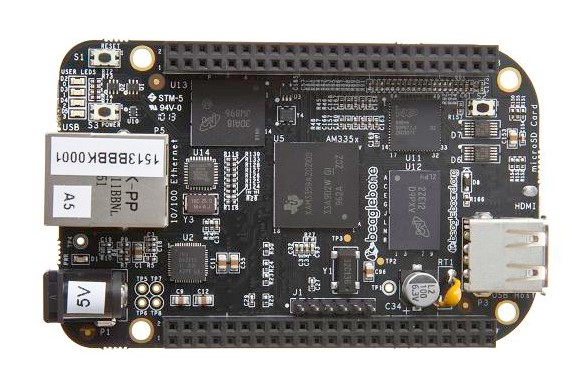
\includegraphics[angle=0,height=5cm]{images/BeagleBoneBlack.jpg}
\caption{Originaler BeagleBone Black}
\label{fig:BeagleBoneBlack}
\end{figure}


\section{Aufgabenstellung}
%Auftrag generell
Im Auftrag des Industriepartners Variosystems soll ein eigener, kostengünstiger und auf dem BeagleBone Black basierter Platinencomputer entwickelt werden. Dafür gilt es, ergänzend zu den eigentlichen Funktionen des BeagleBone Black, weitere Funktionen wie WLAN, Bluetooth Low-Energy, und GSM/GPRS zu integrieren. Zusätzlich soll ein TFT-Display mit einem kapazitivem Multi-Touch-Screen angeschlossen werden, welches von Variosystems zur Verfügung gestellt wird. Das Ganze soll dann als Einheit aufgebaut werden.

%Herstellbarkeit praktisch
Ziel der Arbeit ist es, dass Variosystems diesen Computer selber herstellen und nach Wunsch modifizieren kann. Die Produktionspläne sollen so aufbereitet werden, dass die benötigten PCBs bei einem PCB-Hersteller bestellt werden können. Die Bestückung der PCBs erfolgt dann bei Variosystems. Bei den Bauteilen ist ein besonderes Augenmerk auf die Lieferbarkeit zu werfen. Damit die Bauteile bestellt werden können, muss eine Bauteilliste, auch 'Bill of material' oder kurz BOM, erstellt werden. Diese Liste ist mit der Bestellnummer von üblichen Distributoren wie zum Beispiel Digi-Key oder Mouser zu ergänzen. Standartbauteile, wie etwa Widerstände, hat Variosystems auf Lager. Bei solchen Bauteilen muss auch die Artikelnummer von Variosystems für das entsprechende Bauteil in der BOM aufgeführt werden.

%Modularität, kritischer bereich, 
Die Hardware wie auch die Software sollen möglichst modular aufgebaut sein. Dies bedeutet für die Entwicklung der Hardware, dass alle Bauteile für eine bestimmte Funktion gruppiert und eindeutig erkennbar sein müssen. Ebenso sollen die Bauteile identifiziert werden, welche für die Lauffähigkeit des Computers unbedingt benötigt werden. Ein besonderes Augenmerk ist auf die Stellen zu werfen, bei denen die Leiterbahngeometrie relevant ist. Wie etwa bei der Hochgeschwindigkeitsschnittstelle zwischen Prozessor und RAM. Die Softwaretreiber sollen so geschrieben sein, dass die einzelnen Treiber ohne die anderen lauffähig sind. 

%Software
Zusätzlich zu den Treibern sollten auch Applikationen für die einzelnen Module entwickelt werden. Diese Applikationen sollen als Demonstration der Funktionen und als Vorlage für mögliche Anwendungen verwendet werden können.

	
	\chapter{Einleitung}


\section{Git-Repositories}
Dieses Dokument enthält die gesamte Dokumentation.
Zusätzlich wurden auf drei verschiedenen Git-Repositories entwickelt.

\textbf{Pseudo Sequencer}\\
Der \textit{Pseudo Sequencer} wurde am Anfang der Entwicklung geschrieben, um Zusammenhänge zu verstehen und das ganze Konzept logisch zu verstehen.
Er erhält Code, der C++ ähnelt, ist aber nicht lauffähig.
\begin{itemize}
\item \url{https://github.com/MarcelGehrig2/pseudoSequencer}
\end{itemize}

\textbf{TestApp}
Dieses Repository wurde synchron mit der EEROS-Repository mitentwickelt.
Wenn beim Sequenzer im EEROS-Repository eine neue Funktion eingebaut wurde, wurde sie vor dem Commit mit dieser Testapplikation getestet.
\begin{itemize}
\item \url{https://github.com/MarcelGehrig2/testAppVt1}
\end{itemize}

\textbf{EEROS-Repository}
Das EEROS-Repository ist ein Fork vom originalen EEROS-Repository (Hash: f4d8c8e32c138fdca5d1eb47d6e821c374c2cf07).
In diesem Repository wurde der Sequenzer entwickelt.
\begin{itemize}
\item \url{https://github.com/MarcelGehrig2/eeros-vt1}
\end{itemize}



\section{EEROS}
% kurze beschreibung von eeros
EEROS (Easy, Elegant, Reliable, Open and Safe) ist ein echtzeitfähiges, Open Source Software Framework, welches an der NTB entwickelt wurde und auch immer noch weiter entwickelt wird. 
Das Ziel von EEROS ist, möglichst zuverlässig und einfach in der Bedienung zu sein.
Da das Framework besonders auch in industriellen Robotern zum Einsatz kommen soll, ist besonders auch die Zuverlässigkeit der Software ein wichtiger Punkt.
Für die Software wird die objektorientierte Programmiersprache C++ verwendet. %TODO akronym für sw, besserer satz


EEROS kann in vier Hauptbereiche unterteilt werden.
\begin{enumerate}
\item Die HAL (Hardware Abstraction Layer), welche als Schnittstelle zur Hardware dient.
\item Das CS (\textit{ControlSystem}). Im CS wird die Regelung des Roboters aufgebaut.
In diesem System wird aber nicht nur die Regelung gerechnet, sondern auch Aufgaben wie die Berechnung der Vorwärts- und Inverskinematik werden hier erledigt.
\item Der Sequencer steuert den Ablauf des Roboters.
Hier werden sowohl Wegpunkte aufgelistet, wie auch das allgemeine Verhalten definiert. %TODO besserer satz
\item Im SS (\textit{SafetySystem}) werden sicherheitsrelevante Parameter überwacht. Das SS arbeitet unabhängig vom CS und vom Sequencer. Es löst ein Not-Aus aus, wenn der Roboter ausserhalb der zulässigen Parameter operiert. Ein möglicher Grund für ein Not-Aus wäre zum Beispiel, wenn sich der Roboterarm in einem Sicherheitsbereich zu schnell bewegt.
\end{enumerate}


%TODO bild eeros system




\section{Klarstellung der Benennungen}
% Mischung englisch deutsch
Die meisten Programmiersprachen werden in Englisch codiert.
Auch die offizielle Onlinedokumentation \cite{eerosOrg} von EEROS und die Benennung von Komponenten und Konzepten ist in Englisch.
In diesem Dokument wird an vielen Stellen bewusst darauf verzichtet, englische Bezeichnungen auf Deutsch zu übersetzen.
Dies kann zu Deutsch - Englischen Mischwörter führen.
Solche Mischwörter sind zwar nicht elegant, können aber besser für die Verständlichkeit sein und werden deshalb mit Absicht verwendet.
Auch einige Eigennamen, wie z.B. \textit{Sequencer} anstelle von \textit{Sequenzer}, werden in diesem Dokument nicht immer auf Deutsch übersetzt.

In dieser Arbeit wird oft von drei verschiedenen Kategorien von Entwicklern gesprochen.
Es wird zwischen EEROS-, Steuerungs- und Applikationsentwickler unterschieden.

Der \textbf{EEROS-Entwickler} hat vertiefte Kenntnisse der Programmiersprache C++ und vom EEROS Framework.
Seine Hauptaufgabe ist die Weiterentwicklung des Frameworks, welches vom Steuerungsentwickler verwendet wird.

Der \textbf{Steuerungsentwickler} hat ebenfalls gute C++ Kompetenzen und nutzt das Framework um eine Steuerung für einen Roboter zu entwickeln.
Dafür muss er seine Software speziell an den Roboter anpassen.
Er bereitet auch erste Sequenzen für den Applikationsentwickler vor.
Oft wird die Entwicklung der Steuerung und der Applikation von derselben Person übernommen.

Um den Ablauf des Roboters anzupassen kann der \textbf{Applikationsentwickler} bestehende Sequenzen einfach abändern.
Dazu werden nur grundlegende Programmierfähigkeiten benötigt.
Mit etwas erweiterten Kenntnissen kann er auch neue Sequenzen erstellen.



\section{Aufgabenstellung}
In der aktuellen Version von EEROS existiert bereits eine erste Version von einem Sequencer.
Dieser ist in seiner Funktionalität und Übersichtlichkeit aber stark eingeschränkt.
Oft musste auf Tricks zurückgegriffen werden, damit bestimmte Aufgaben mit dem bestehenden Sequencer gelöst werden konnten.
Um eine bestehende Sequenz anpassen zu können, auch wenn der Ablauf nur geringfügig geändert werden soll, ist schon viel Fachwissen notwendig.

In dieser Vertiefungsarbeit sollen diese beiden Probleme gelöst werden.
Es soll ein neuer Sequencer entwickelt werden, der flexibel für verschiedenste Arten von Robotern eingesetzt werden kann.
Die Sequenzen, welche den Ablauf des Roboters beschreiben, sollen dabei möglichst einfach und übersichtlich aufgebaut sein.
Dank des einfachen Aufbaus soll es auch für einen Applikationsentwickler möglich sein Sequenzen anzupassen und zu erstellen, auch wenn er keine vertieften Kenntnisse von C++ besitzt.

% vorgehen: requirement, konzept, ausarbeitung, implementierung
	\chapter{EEROS aktueller Stand}
\section{EEROS generell}
%TODO


\section{Aktuelle Implementierung des Sequencers}
Für EEROS besteht bereist ein rudimentärer \textit{Sequencer}.
Im folgenden Kapitel wird die bestehende Implementierung kurz erklärt.
In der Onlinedokumentation\footnote{http://wiki.eeros.org/eeros\_architecture/sequencer/start} wird noch vertiefter in die Details des bestehenden \textit{Sequencers} eingegangen, als in dieser Arbeit.


\subsection{Sequencer}
Die Grundlage bildet ein Sequencer-Objekt, das in einem Nicht-Realtime-Thread läuft.
In so einem \textit{Sequencer} können eine Serie von blockierenden \textit{Sequences} aufgerufen werden.
Wenn mehrere parallele \textit{Sequences} aufgerufen werden sollen, muss für jede \textit{Sequence} ein eigener \textit{Sequencer} erstellt werden.

\begin{figure}[!ht]
\centering
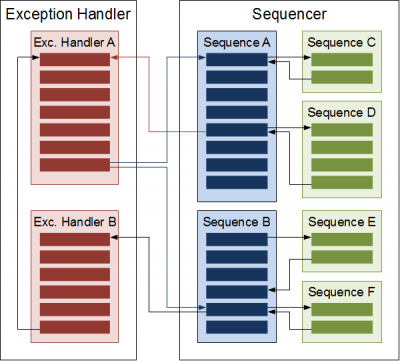
\includegraphics[angle=0,height=8cm]{images/SequencerBestehend.png}
\caption{Schematische Darstellung des bestehenden Sequencers \protect\footnote{http://wiki.eeros.org/eeros\_architecture/sequencer/start}}
\label{sequencerBestehend}
\end{figure}


\subsection{Sequence}
Eine \textit{Sequence} führt als erstes eine benutzerdefinierte Initialisierungsfunktion aus.
Als nächstes wird eine \textit{preCondition} überprüft.
Fehlt die Überprüfung fehl, wird die \textit{Sequence} abgebrochen.
Bei einem positiven Ergebnis wird der Hauptteil, eine Abfolge von definierten \textit{Steps} ausgeführt.
Dem letzten \textit{Step} folgt noch eine Überprüfung einer \textit{postCondition}.
Läuft der \textit{Sequencer} im \textit{stepping-mode}, wird die \textit{Sequence} bei jeden \textit{yield()} pausiert und wird erst fortgeführt, wenn der Befehl dazu gegeben wird.\footnote{http://wiki.eeros.org/eeros\_architecture/sequencer/start}

\begin{lstlisting}
init();
yield();

if(!checkPreCondition()) 
  return SequenceResult<void>(result::preConditionFailure);
yield();

run();
yield();

if(!checkPostCondition())
  return SequenceResult<void>(result::postConditionFailure);
yield();

exit();
return SequenceResult<void>(result::success);
\end{lstlisting}


\subsection{Step}
Ein \textit{Step} ist eine vom \textit{Steuerungsentwickler} festgelegte Einheit, die von einem \textit{yield()} Befehl unterteilt wird.
\textit{Steps} können im \textit{stepping-mode} einzeln abgearbeitet werden.


\subsection{Sub-Sequence}
\textit{Subsequences} sind sehr ähnlich wie normale \textit{Sequenzen}.
Sie können verwendet werden, wenn ein ähnlicher Ablauf mehrmals wiederholt werden soll.
Durch eine Übergabe von Parameter an eine solche \textit{Subsequence} kann sie sehr flexibel gestaltet werden.
Wenn die \textit{Subsequence} parallel, also nicht-blockierend, aufgerufen werden soll, muss sie einem neuen Sequencer übergeben werden.

\begin{lstlisting}
class SequenceB : public Sequence<> {
public:
  SequenceB(std::string name, Sequencer* seq, Robot& r) : Sequence<void,double>(name, seq), robot(r){ }
 
  void run() {
    robot.moveZ(5);
    sleep(3);
    yield();
    robot.moveZ(0);
  }
 
private: 
  Robot& robot;
};
\end{lstlisting}


\subsection{Error-Handler}
Der \textit{Error-Handler} wird in der Onlinedokumentation zwar erwähnt, im Sourcecode von EEROS sind aber keine Spuren von der Implementierung zu finden.
Der Dokumentation zu folge soll er \textit{Exceptions} behandeln.
Je nach \textit{Exception} soll er flexibel reagieren, um Probleme zu beheben.



%\section{Fallbeispiel Parallel Scara}
%
%\begin{figure}[!ht]
%\centering
%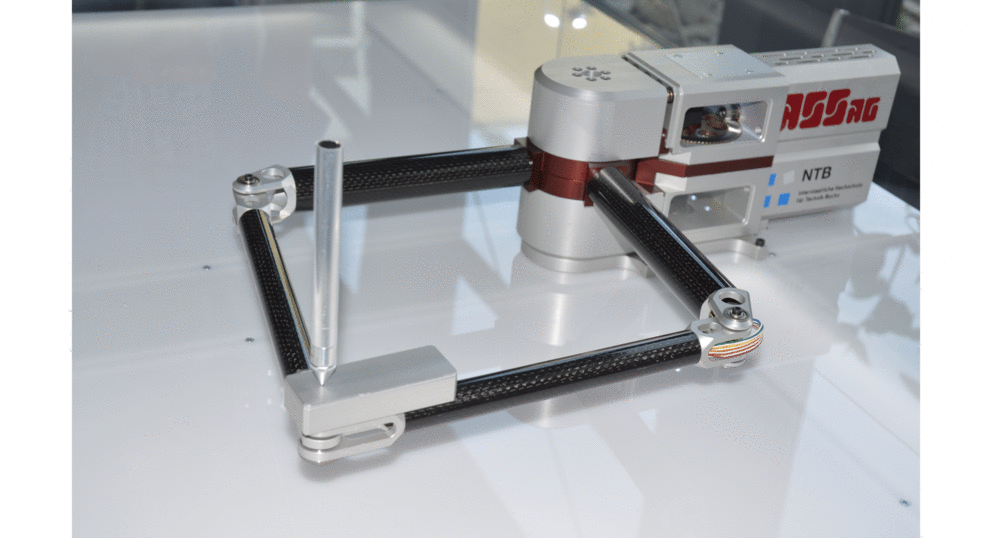
\includegraphics[angle=0,height=8cm]{images/ParallelScara.png}
%\caption{Der Parallel Scara Roboter \protect\footnote{http://www.ntb.ch/projekt/parallel-scara/}}
%\label{parallelScara}
%\end{figure}
%
%Der Parallel Scara ist ein Roboter, dessen Hardware und auch Software an der NTB entwickelt wurde.
%Die Steuerung ist mit EEROS und dem bestehenden \textit{Sequencer} aufgebaut.
%Im folgenden Kapitel wird der Quellcode der Steuerung analyisiert um herauszufinden, welche Aspekte des bestehenden \textit{Sequencers} brauchbar sind, und wo er noch Lücken aufweist.
%
%
%\subsection{asdf}



\section{Fallbeispiel 'EEDURO Delta Roboter'}

%\begin{figure}[!ht]
%\centering
%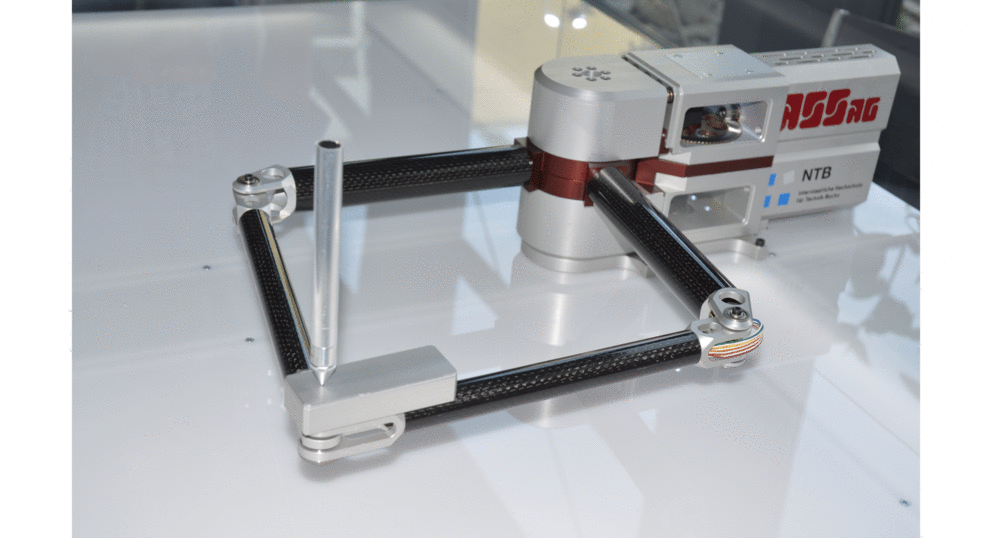
\includegraphics[angle=0,height=8cm]{images/ParallelScara.png}
%\caption{Der Parallel Scara Roboter \protect\footnote{http://www.ntb.ch/projekt/parallel-scara/}}
%\label{parallelScara}
%\end{figure}

Der \textit{EEDURO Delta Roboter} ist ein Roboter, dessen Hardware und auch Software an der NTB entwickelt wurde.
Die Steuerung ist mit EEROS und dem bestehenden \textit{Sequencer} aufgebaut.
Im folgenden Kapitel wird der Quellcode der Steuerung analyisiert um herauszufinden, welche Aspekte des bestehenden \textit{Sequencers} brauchbar sind, und wo er noch Lücken aufweist.

Der Quellcode der Steuerungssoftware ist auf folgendem Git-Repository zu finden: \\
\textit{https://github.com/ClaudiaVisentin/eeduro-platform }

%Die Software wurde vom Stand 10.10.2016 mit folgendem Hashverwendet: \\ \textit{a25bcfa752516723f067f5a5166e8f09e60fc6e8}
Die Software wurde vom Stand 10.10.2016 mit dem Hash \textit{\seqsplit{a25bcfa752516723f067f5a5166e8f09e60fc6e8}} verwendet.


\subsection{asdf}

	\chapter{Anforderungen an den Sequencer}
%TODO wie wurden ziele ausgearbeitet
\section{Formulierung der Anforderungen}
Im folgenden Kapitel werden die Anforderungen an den \textit{Sequencer} beschrieben.
Die Kapitel \textit{Ziele}, \textit{Nicht Ziele} und \textit{Test Cases} beschreiben die Anforderungen auf verschiedene Arten.
In \textit{Ziele} und \textit{Nicht Ziele} wird abstrakt beschrieben, welche Funktionen der neue \textit{Sequencer} beinhalten, beziehungsweise nicht beinhalten muss.
Im Kapitel \textit{Test Cases} werden verschiedene Fälle beschrieben die mit dem neuen \textit{Sequencer} möglichst elegant gelöst werden sollen.



\section{Ziele}
\subsection{Einfaches Interface für den Applikationsentwickler}
Mit dem bestehenden \textit{Sequencer} sind vertiefte Programmierkenntnisse notwendig, um eine Sequenz zu erstellen, oder abzuändern.
Sequenzen sind nicht intuitiv verständlich.
Es werden Kenntnisse vom \textit{Control System} und dem \textit{Safety System} benötigt, um einen neuen Ablauf für den Roboter schreiben zu können. %TODO Satz
Zurzeit werden Sequenzen von den Steuerungsentwickler geschrieben.

Wenn der Roboter fertig entwickelt worden ist, soll er an einen Kunden übergeben werden können.
Der Kunde, oder der Betreiber des Roboters, soll dann Änderungen im Ablauf des \textit{Sequencers} vornehmen können, ohne dass er vertiefte Kenntnisse von der Programmiersprache C++ oder von der inneren Funktionsweise des Roboters haben muss.
Dafür ist es notwendig, dass der Steuerungsentwickler den Roboter so abstrahiert, dass die Sequenzen aus logischen und verständlichen Schritten bestehen.


\subsection{Flexibel einsetzbar für verschiedenste Arten von Roboter}
Auch wenn die Sequenzen möglichst einfach aufgebaut werden sollen, muss der \textit{Steuerungsentwickler} für alle möglichen Kategorien von Robotern Sequenzen bauen können.
Verschiedene Arten von Roboter haben verschiedene Anforderungen.
Das \textit{Control System} von einem Roboterarm mit sechs Freiheitsgraden unterscheidet sich stark von einer Fertigungsstrassen mit mehreren Förderbändern.
Trotz diesen Unterschieden soll es möglich sein, für beide Kategorien von Robotern sinnvolle Sequenzen zu erstellen.
Das bedeutet, dass der \textit{Steuerungsentwickler} möglichst viele Freiheiten beibehält, ohne dass er durch das \textit{Framework} unnötig begrenzt wird.
%TODO ss missbraucht


\subsection{Parallele und blockierende Sequenzen}
Wie bereits im bestehenden Sequenzer verwirklicht wurde, sollen Sequenzen blockierend und nicht-blockierend aufgerufen werden können.
Diese Funktion von blockierenden und parallel ausgeführten Sequenzen soll auch im neuen \textit{Sequencer} beibehalten werden.
 

\subsection{Exception Handling}
Eine \textit{Exception} ist ein Ereignis, dass nicht immer auftritt, aber auftreten kann.
Zu solchen \textit{Exception}, oder Ausnahmen, gehören zum Beispiel:
\begin{enumerate}
\item Ein blockiertes Förderband
\item Ein Timeout
\item Der Roboter soll ein Paket abholen, dass nicht vorhanden ist
\end{enumerate}
Solche Ausnahmen sollen im \textit{Sequencer} erkennt werden können und flexibel darauf reagiert werden können.
Eine solche Reaktion könnte eine spezielle Sequenz sein, die versucht, eine solche Ausnahme zu behandeln.
Alternativ soll aber auch die aktuelle Sequenz abgebrochen, oder neu gestartet werden können.


\subsection{Zugriff auf Control System}
Der aktuelle \textit{Sequencer} nutzt ein Pointer auf das \textit{Control System} um Blöcke direkt auslesen und schreiben zu können.
Wenn das \textit{Control System} betrachtet wird, kann nicht festgestellt werden, welche Blöcke vom \textit{Sequencer} ausgelesen oder geschrieben werden.
Ein klares Interface zum \textit{Sequencer} wäre wünschenswert, um das \textit{Control System} übersichtlicher zu machen.


\subsection{Safety System entlasten}
Eine Analyse von bestehenden Implementationen des alten \textit{Sequencers} hat gezeigt, dass das \textit{Safety System} viele Aufgaben übernimmt, welche besser vom \textit{Sequencer} übernommen werden sollten.
Das \textit{Safety System} sollte möglichst nur eingesetzt werden, um das System zu überwachen.
Alle anderen Aufgaben sollen vom \textit{Sequencer} oder vom \textit{Control System} übernommen werden.



\section{Nicht Ziele}
\subsection{Echtzeit}
Das \textit{Control System} und das \textit{Safety System} laufen beide in einem Echtzeit-Task.
Der \textit{Sequencer} soll aber bewusst nur mit normaler Priorität laufen und besitzt keine Echtzeit Fähigkeit.

Da der \textit{Sequencer} keine Regelung berechnet, benötigt er keine Echtzeit Fähigkeit.
Eine niedrigere Priorität als das \textit{Control System} und das \textit{Safety System} ist notwendig, dass die beiden Systeme nicht vom \textit{Sequencer} beeinträchtigt werden.


\subsection{Pfadplanung}
Die Pfadplanung ist nicht Teil des \textit{Sequencers}, da sie den Rahmen dieser Arbeit sprengen würde.



\section{Test Cases}
\subsection{Einleitung}
Die Testfälle sind so aufgebaut, dass sie möglichst einfach und elementar sind.
Jeder \textit{Test Case} beschreibt eine andere Anforderung oder Spezialfall an den \textit{Sequencer}.
Alle in der Realität vorkommenden Situation sollte durch einen, oder einer Kombination von mehreren, \textit{Test Cases} beschrieben werden können.

Eine Ausnahme dazu bildet \textit{Test Case 8}.
In diesem Testfall wurden möglichst viele verschiedene Situationen vereint.

Mit dem \textit{Sequencer} sollen alle Testfälle sauber und elegant umgesetzt werden werden können.


\subsection{Test Case 1: Achse einfach}
\textbf{System}
\begin{itemize}
\item Eine Achse die sich nach links und rechts bewegen kann
\item An beiden Enden befindet sich ein Endschalter
\item Ein Taster \textit{Taster links}, der die Achse nach links laufen lässt
\item Ein Taster \textit{Taster rechts}, der die Achse nach rechts laufen lässt
\end{itemize}

\textbf{Aufgabe}
\begin{itemize}
\item Solange \textit{Taster links} gedrückt bleibt, fährt die Achse nach links
\item Solange \textit{Taster rechts} gedrückt bleibt, fährt die Achse nach rechts
\item Die Achse hält an, wenn einer der beiden Endschalter erreicht wird
\end{itemize}

\textbf{Herausforderungen}
\begin{itemize}
\item Der \textit{Sequencer} muss die Eingänge \textit{Taster links}, \textit{Taster rechts} und die beiden Endschalter permanent überwachen und auf eine Änderung reagieren.
\end{itemize}


\subsection{Test Case 2: EEDURO Delta Roboter Maus}
\textbf{System}
\begin{itemize}
\item EEDURO Delta Roboter mit Maus
\end{itemize}

\textbf{Aufgabe}
\begin{itemize}
\item Während dem Idle Zustand wird auf einen Input von der Maus gewartet
\item Wenn sich die Maus für fünf Sekunden nicht bewegt, wird eine blockierende \textit{Autor-Sort Sequenz} gestartet
\item Bewegt sich die Maus innerhalb von fünf Sekunden, dann bewegen sich die Achsen entsprechend der Mausbewegung und der 5-Sekunden-Timer wird neu gestartet
\end{itemize}

\textbf{Herausforderungen}
\begin{itemize}
\item Timeout
\item Blockierende Sequenz
\end{itemize}


\subsection{Test Case 3: Rendezvous}
\textbf{System}
\begin{itemize}
\item Greifer Zubringer
\item Greifer Abholer
\item Paket: Gegenstand, der übergeben wird
\item Förderband Zubringer: Hält ständig ein neues Paket bereit für \textit{Greifer Zubringer}
\item Förderband Abholer: Transportiert ständig alle Pakete weg, welche vom \textit{Greifer Abholer} abgelegt werden
\end{itemize}

\textbf{Ablauf (Siehe Abbildung \ref{Testcase03Picture}})
\begin{enumerate}
\item Der \textit{Greifer Zubringer} holt ein neues Paket vom \textit{Förderband Zubringer}
\item Der \textit{Greifer Zubringer} bringt das Paket in Rendezvous-Position
\item Der \textit{Greifer Abholer} übernimmt das Paket vom \textit{Greifer Zubringer} 
\item Der \textit{Greifer Abholer} legt das Paket auf das \textit{Förderband Abholer}
\item Die Sequenz beginnt wieder von Anfang an
\end{enumerate}

%\begin{figure}[!ht]
\begin{figure}[]
\centering
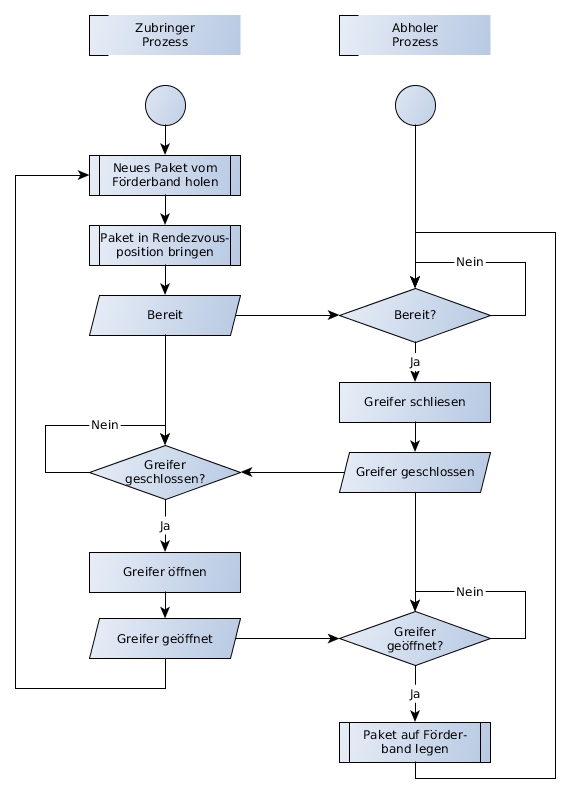
\includegraphics[angle=0,height=10cm]{images/Testcase03.png}
\caption{\textit{Test Case 3}: Ablaufdiagramm vom}
\label{Testcase03Picture}
\end{figure}

\textbf{Herausforderungen}
\begin{itemize}
\item Synchronisation von zwei parallellaufenden Sequenzen
\item Kommunikation zwischen zwei Sequenzen
\end{itemize}


\subsection{Test Case 4: Sequenz pausieren}
\textbf{System}
\begin{itemize}
\item Roboterarm
\item Ein Taster \textit{Taster Pause}, der die Sequenz pausiert
\end{itemize}

\textbf{Ablauf}
\begin{itemize}
\item Der Roboterarm führt eine sich wiederholende Sequenz endlos aus
\item Wird \textit{Taster Pause} gedrückt, pausiert die Sequenz
\item Wird \textit{Taster Pause} erneut gedrückt, wird die Sequenz fortgeführt
\end{itemize}

\textbf{Herausforderungen}
\begin{itemize}
\item Jede Sequenz muss jederzeit pausiert werden können
\item Der Taster gibt nur einen Impuls, nicht eine bleibende Pegeländerung an einem Eingang
\item Timeouts müssen pausiert werden
\end{itemize}


\subsection{Test Case 5: Zwei Roboterarme}
\textbf{System}
\begin{itemize}
\item Roboterarm A
\item Roboterarm B
\item Ein Taster \textit{Taster Pause}, der beide Sequenzen pausiert
\end{itemize}

\textbf{Ablauf}
\begin{itemize}
\item Beide Roboterarme führen sich wiederholende Sequenz endlos aus
\item Wird \textit{Taster Pause} gedrückt, pausieren beide Sequenzen
\end{itemize}

\textbf{Herausforderungen}
\begin{itemize}
\item Zwei parallellaufende Sequenzen müssen mit einem Taster pausiert werden können
\end{itemize}


\subsection{Test Case 6: Prellender Taster}
\textbf{System}
\begin{itemize}
\item Ein prellender Taster \textit{Taster A}
\end{itemize}

\textbf{Aufgabe}
\begin{itemize}
\item Ein prellender Taster soll sauber eingelesen werden
\end{itemize}

\textbf{Herausforderungen}
\begin{itemize}
\item Der Taster muss entprellt werden
\item Mehrmaliges drücken soll sauber registriert werden, auch wenn der Taster in schneller Abfolge gedrückt wird
\end{itemize}

\begin{figure}[]
\centering
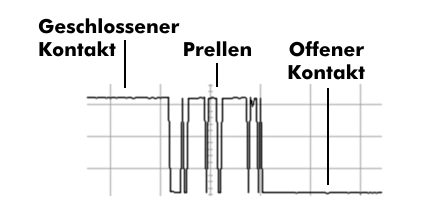
\includegraphics[angle=0]{images/Testcase06.png}
\caption{\textit{Test Case 6}: Signalverlauf bei einem prellenden Schalter}
\label{Testcase06Picture}
\end{figure}


\subsection{Test Case 7: Menü}
\label{Testcase07}
\textbf{System}
\begin{itemize}
\item Ein beliebige Anzahl Taster \textit{Taster A}, \textit{Taster B}, \textit{Taster C}, ....
\end{itemize}

\textbf{Aufgabe}
\begin{itemize}
\item Wenn sich das System in einem \textit{Idle} Zustand befindet, soll jeder Taster eine andere Sequenz starten
\end{itemize}

\textbf{Herausforderungen}
\begin{itemize}
\item Dieses \textit{Menü} lässt sich nicht im klassischen Sinne als eine Sequenz, also eine Abfolge von Schritten, beschrieben werden. Trotzdem soll eine einfache Implementierung im \textit{Sequencer} möglich sein
\end{itemize}


\subsection{Test Case 8: Detailliertes Rendezvous}
Dieser \textit{Test Case} basiert auf auf dem \textit{Test Case 3}, ist aber detaillierter ausgearbeitet.
Im Anhang \ref{sec:anhang_test_case_8} ist das Ablaufdiagramm der Hauptsequenz \textit{Sequenz Rendezvous} und der blockierenden Subsequenz \textit{Sequenz PickUp} angehängt.
Das Ziel von diesem \textit{Test Case} war es nicht einen realistischen Fall abzubilden.
Viel mehr dient er dazu, möglichst viele Fälle und Situationen abzubilden, die in einer Sequenz vorkommen können.

%TODO grundlage für diskus

Das Ablaufdiagramm besteht aus folgenden Blöcken:
\begin{itemize}
\item Rechtecke: einzelne Steps
\item Rechtecke mit doppelten, vertikalen Linien: Blockierende Subsequenzen
\item Blaue Rauten: Entscheidungen
\item Grüne Rauten: Blockierungen, bis Entscheidung wahr wird
\item Parallelogramm: Statusvariable wird geändert
\item Lange senkrechte Rechtecke: Bedingung, welche über längere Zeit überwacht wird
\end{itemize}




%	\chapter{Dokumentation für Steuerungsentwickler}
Dieses Kapitel ermöglicht einen leichten Einstig in den neuen Sequencer.
Es deckt aber nicht vollständig alle Details von allen Funktionen des Sequencer ab.
Eine detailliertere Beschreibung des Sequencers und von dessen Funktionen findet sich im Kapitel \ref{sequencerAufbau}.


\section{Den Sequencer erstellen}
Im Hauptprogramm der Applikation muss der Sequenzer erst erstellt werden.
Die Hauptsequenz, in diesem Beispiel \textit{mainSequence} genannt, wird in einem Thread gestartet, sobald sie dem Sequencer hinzugefügt wird.
Alle anderen Sequenzen werden von der Hauptsequenz aus gestartet.

\textit{main.cpp:}\
\begin{lstlisting}
#include "sequences/MainSequence.hpp"

eeros::sequencer::Sequencer S;
MainSequence mainSequence(S, &controlSystem, "mainSequence");
S.addMainSequence(&mainSequence);

executor.run();
mainSequence.join();	//The application only stops, when the mainSequence is finished
\end{lstlisting}


\section{Benutzerdefinierte Sequenz}
\subsection{Eigenschaften von Sequenzen}
Sequenzen werden standardmässig nicht-blockierend gestartet.
Es besteht aber auch die Möglichkeit, Sequenzen blockierend zu starten.


\subsection{Vorteile von benutzerdefinierten Sequenzen}



\subsection{Beispiel für eine mainSequence}

\textit{MainSequence.hpp:}\
\begin{lstlisting}
#include "SequenceA.hpp"
#include "SequenceB.hpp"
#include "SequenceExceptionA.hpp"

namespace testappsequencer {

	class TestAppCS;
	
	class MainSequence : public eeros::sequencer::Sequence {
	public:
		MainSequence(Sequencer& S, TestAppCS* CS, std::__cxx11::string name);

		int action();
		
		SequenceA seqA1;
		SequenceB seqB1; 
		SequenceB seqB2; 
		SequenceB seqB3;
		
		SequenceExceptionA seqEA1;
		
		TestAppCS* CS;
	};
};
\end{lstlisting}

Jede Sequenz muss von der Klasse \textit{eeros::sequencer::Sequence} abgeleitet werden.

\textbf{Zeile 7} und \textbf{Zeile 22} sind notwendig, um einen Pointer auf das \textit{ControlSystem} zu erhalten.
Dafür muss zusätzlich der \textit{Constructor} angepasst werden.

\textit{int action();} ist die wichtigste Methode der Sequenz.
Sie beinhaltet den Ablauf der Sequenz.

\textbf{Zeile 15} bis \textbf{Zeile 20} beschreiben benutzerdefiniert Sequenzen, die von der Hauptsequenz aus gestartet werden.


\textit{MainSequence.cpp:}\
\begin{lstlisting}
#include "MainSequence.hpp"

using namespace testappsequencer;
using namespace eeros;
using namespace eeros::sequencer;


MainSequence::MainSequence(Sequencer& S, TestAppCS* CS, std::__cxx11::string name) :
Sequence(S, name), CS(CS),

seqA1(S, CS, this, "seqA1"),
seqB1(S, CS, this, "seqB1"),
seqB2(S, CS, this, "seqB2"),
seqB3(S, CS, this, "seqB3"),
seqEA1(S, CS, this, "seqEA1")		//Exception Sequence
{
	setIsNonBlocking();
	
	seqA1.setTimeoutTime(5.1);
	seqA1.setTimeoutExceptionSequence(&seqEA1);
	seqA1.setTimeoutBehavior(restartOwner);
	
	seqA1.setIsBlocking();
}

int MainSequence::action()
{
	seqB1();
	seqB2();
	seqA1(10, 3);
	seqB3();
	
	seqB1.join();
	seqB2.join();
	seqB3.join();
	
	log.info() << "MainSequence ended";
}
\end{lstlisting}

In \textbf{Zeile 9} wird die Basis-Sequenz und der Pointer für das \textit{ControlSystem} initialisiert.
Zusätzlich müssen auch alle Sequenzen, die in dieser Sequenz genutzt werden, initialisiert werden.

\textbf{Zeile 17} definiert diese Sequenz als nicht-blockierend.
Die Hauptsequenz von einer Applikation muss immer nicht-blockierend sein.
Andere Sequenzen können blockierend sein.

Die \textbf{Zeile 19} aktiviert für die Sequenz \textit{seqA1} den Timeout und setzt die Zeit auf 5.1 Sekunden.
Wenn \textit{seqA1} nach 5.1 Sekunden Laufzeit noch nicht fertig abgearbeitet wurde, wird \textit{seqEA1} ausgeführt.
Nachdem die Exception-Sequenz \textit{seqEA1} beendet wurde, wird \textit{seqA1} neu gestartet, da dieses Verhalten in \textbf{Zeile 21} definiert wurde.

Durch den Befehl in \textbf{Zeile 23} wird \textit{seqA1}, unabhängig vom vordefinierten Standard von \textit{SequenceA}, blockierend ausgeführt.

In der Methode \textit{action()} wird der eigentliche Ablauf von der Sequenz definiert.
Als erstes wird \textit{seqB1} gestartet.
Da sie, und auch \textit{seqB2}, nicht-blockierend sind, wird sofort auch \textit{seqB2} und \textit{seqA1} gestartet.
Weil \textit{seqA1} den weiteren Ablauf blockiert, bis sie fertig gestellt wurde, wird \textit{seqB3} erst ausgeführt, wenn \textit{seqA1} beendet wurde.

Mit den \textit{join()}-Befehlen kann sichergestellt werden, dass die Hauptsequenz erst dann beendet wird, wenn die entsprechenden, parallel laufenden Sequenzen fertig abgearbeitet wurden.


\subsection{Beispiel für eine benutzerdefinierte Sequenz 'SequenceA'}

\textit{SequenceA.hpp:}\
\begin{lstlisting}
#include "SequenceExceptionA.hpp"

namespace testappsequencer {
	
	using namespace eeros::sequencer;
	
	class TestAppCS;
	
	class SequenceA : public Sequence {
	public:
		SequenceA(Sequencer& S, TestAppCS* CS, BaseSequence* caller, std::__cxx11::string name);
		
		int operator()(int a, int b);
		//int operator()(std::string str);
		//int operator()();
		int action();
		
		SequenceExceptionA seqEA2;
		
		TestAppCS* CS;
		int posA;
		int posB;
	};
};
\end{lstlisting}

Der Aufbau von dieser Sequenz ähnelt stark dem Aufbau von der Hauptsequenz.
Der einzige Unterschied ist die Methode \textit{int operator()(int a, int b);}.
Diese Methode wird aufgerufen, bevor die Sequenz gestartet wird und kann genutzt werden, um Parameter zu übergeben.
Je nach Bedarf können die Typen und Anzahl der Parameter frei gewählt werden, oder mit \textit{int operator()();} ganz weggelassen werden.


\textit{SequenceA.cpp:}\
\begin{lstlisting}
#include "SequenceA.hpp"
#include "../steps/StepA.hpp"

using namespace testappsequencer;


SequenceA::SequenceA(Sequencer& S, TestAppCS* CS, BaseSequence* caller, std::__cxx11::string name)
: Sequence(S, caller, name), CS(CS),

seqEA2(S, CS, this, "seqEA2Step")
{
	setIsBlocking();
}


int SequenceA::operator()(int a, int b)
{
	posA = a;
	posB = b;
	return Sequence::start();	//this code is mandatory for every derived Step- and Sequence-Class
}


int SequenceA::action()
{
	//initialisation of the step 'goTo'
	GoTo goTo = StepA(S, CS, this);
	sA.setTimeoutTime(5);
 	sA.setTimeoutBehavior(abortOwner);
	sA.setTimeoutExceptionSequence(&seqEA2);
	
	//start of the sequence
	goTo(0);
	goTo(posA);
	goTo(posB);
}

\end{lstlisting}

Mit dem Befehl \textit{setIsBlocking()} im Konstruktor werden standardmässig alle Sequenzen von der Klasse \textit{SequenceA} blockierend ausgeführt.
Der Befehl \textit{seqA1.setIsBlocking();} aus \textit{MainSequence.cpp} wäre somit gar nicht notwendig.

Es ist zwingen notwendig, dass die Methode \textit{operator()} implementiert wird.
Ebenfalls erforderlich ist, dass der letzte Befehl von dieser Methode \textit{return Sequence::start();}  lautet.
Wenn der Sequenz Parameter übergeben werden, dann können hier die Variablen gespeichert werden.

Am Anfang der \textit{action()}-Methode wird ein neuer \textit{Step} initialisiert.
\textit{Steps} verhalten sich sehr ähnlich wie Sequenzen.
Sie können aber nur blockierend aufgerufen werden.
Da \textit{Steps} keinen eigenen Thread starten, brauchen sie weniger Ressourcen und können einfach mehrmals hintereinander aufgerufen werden.



\subsection{Beispiel für einen benutzerdefinierten Step 'GoTo'}

\textit{GoTo.hpp:}\
\begin{lstlisting}
#include <eeros/sequencer/Step.hpp>

namespace testappsequencer {
	
	using namespace eeros::sequencer;
	
	class  TestAppCS;
	
	class GoTo : public Step {
	public:
		GoTo(Sequencer& S, TestAppCS* CS, BaseSequence* caller);
		
		int operator()(int a, int b);
		int action();
		bool checkExitCondition();
		
		TestAppCS* CS;
	};

	
	
};
\end{lstlisting}
%	\include{DokumentationFuerApplikationsentwickler}
	\chapter{Aufbau des Sequencers}


\section{Caller Stack}
Das unterste (älteste) Element ist die ID-Nummer der Hauptsequenz.
Als nächstes folgt 
 %innerer Aufbau
%	\chapter{Test des Sequencer}


\section{section}
%	\chapter{Ergebnis, Fazit und Ausblick}
\section{Ergebnis}
Der entwickelte Sequenzer löst viele Probleme des alten Sequenzer.
Es ist nun möglich Sequenzen so zu bauen, dass sie auch für Nicht-Experten einfach verständlich sind.

Die Klasse \textit{Condition} erlaubt es nun, komplexe zusammenhängende Zustände in einer Klasse zu Abstrahieren.
Der \textit{Steuerungsentwickler} kann eine benutzerdefinierte Klasse ableiten, die der \textit{Applikationsentwickler} nutzen kann, ohne dass er die implementierte Funktionalität verstehen muss.
Der selbe Vorteil besteht auch für \textit{Sequenzen} und \textit{Steps}.

Mit den neuen \textit{Monitore} existiert eine einfache Möglichkeit, bestimmte Zustände permanent und automatisch zu überwachen.
Die \textit{Monitore} können zusammen mit den \textit{Conditions} als Exception-Handler verwendet werden.

Eine Synchronisation und Datenaustausch zwischen mehreren parallel laufenden Sequenzen ist einfach möglich, da jetzt nur noch der Namen der gesuchten Sequenz bekannt sein muss, um einen Pointer auf die Sequenz zu erhalten.


\section{Fazit}	%subjektiv
Ich habe sehr viel Zeit für den Pseudo-Sequenzer aufgewendet.
Der Plan, den Sequenzer mit Hilfe des Pseudo-Sequnzers genau durchzuplanen und ihn dann in das Framework zu integrieren, ist aber nicht aufgegangen.
Bei der Integration ins EEROS habe ich gemerkt, dass viele Konzepte nicht so funktionierten, wie ich es geplant hatte.
Einige Teile konnte ich mit aufwändig in kleinen Schritten integrieren, andere Teile musste ich verwerfen und neu durchdenken, weil sie nicht möglich waren.

Die vielen unvorhergesehenen Komplikationen haben meinen Zeitplan durcheinander gebracht.
Aus diesem Grund konnte ich die Software nicht ausgiebig testen.

In dieser Arbeit habe ich nicht nur vieles neues Wissen bezüglich der Programmiersprache C++ aneignen, ich habe auch eine Lektion in Software-Management gelernt.
Für Software eignet sich der Ansatz, erst alles durchplanen, dann alles integrieren und am Schluss die komplette Software durchtesten, nicht gut.
In meinem nächsten Software-Projekt werde ich viel mehr auf kleine, aber dafür viele Iterationen planen-implementieren-testen setzen.
Diese Strategie habe ich bei dieser Arbeit leider erst am Schluss eingesetzt.
Besonders auf das Testen werde ich bei der nächsten Arbeit grösseren Wert legen.


\section{Ausblick}
Der neue Sequenzer bildet eine gute Grundlage für einfach verständliche Abläufe mit sehr hoher Flexibilität.
Allerdings wurde er noch nicht ausgiebig getestet, so dass keine Aussage über die Zuverlässigkeit gemacht werden kann.

Des weiteren gibt es noch einige offene Punkte:
\begin{itemize}
\item Genau überprüfen, ob alle Ziele erreicht wurden.
\item Race-Condition. Zum Beispiel wenn mehrere parallel laufende Sequenzen auf das \textit{SafetySystem} oder das \textit{ControlSystem} zugreifen wollen.
\item Geregelter Zugriff auf das \textit{ControlSystem}. Evt. wird von einer Sequenz exklusiven Zugriff auf Teile des \textit{ControlSystem} verlangt, so dass sie nicht von einer anderen Sequenz gestört wird.
\item Onlinedokumentation auf der EEROS-Homepage nachführen.
\end{itemize}

	
	
%	\chapter{Lösungsansätze und Varianten}


\section{Strategie}
% möglichst einfach, sicher funktioniern
Das ganze Projekt inklusive BBB und den diversen Zusatzfunktionen ist technisch sehr komplex. Deshalb wurde beim Variantenentscheid wie auch später in der Planung, besonders darauf geachtet, dass die gewählten Lösungen eine möglichst geringe Fehleranfälligkeit haben. Dies führte auch zu einigen Kompromissen, die im Folgenden erläutert werden.

%TODO massenfertigung

Verschiedene Lösungsansätze wurden bereits im Vorfeld zu dieser Arbeit im Fachmodul gesucht und bewertet. Der Bericht zu diesem Fachmodul befindet sich im Anhang unter dem Kapitel \ref{sec:anhang_pflichtenheft}. Im Fachmodulbericht wird ausführlich auf die verschiedenen Varianten für WLAN, GSM/GPRS und BLE eingegangen. Aus diesem Grund werden hier nur noch die Entscheidungen kurz zusammengefasst und um einige zusätzliche Informationen ergänzt.



\section{Grundsätzlicher Aufbau}
Für den grundsätzlichen Aufbau des ganzen Systems boten sich zwei verschiedene Varianten an. Bei der ersten Variante wird der BBB zusammen mit den Zusatzfunktionen auf einer Platine verwirklicht. Bei der zweiten Variante werden die Zusatzfunktionen auf einem zweiten PCB als Cape aufgebaut.

\subsection{Variante 1: Eine grosse Platine}
Das ganze System, also der BBB und die Bauteile für die Zusatzfunktionen, werden auf einer einzigen Platine platziert.

Vorteile:
\begin{itemize}
\item Alles ist in einem einzigen, geschlossenen Projekt. Dies hat den Vorteil, dass nur ein grosses PCB bestellt und bestückt werden muss. Dies ist kostengünstiger und einfacher als zwei separate PCBs. So muss zum Beispiel die Pick-and-Place-Maschine nur einmal eingerichtet werden.
\item Flexible Form des PCB. Je nachdem wie die Bauteile platziert werden, kann die Form des PCB beeinflusst werden.
\item Die relativ teuren Steckverbindungen zwischen den Platinen fallen weg.
\end{itemize}

\subsection{Variante 2: Die Zusatzfunktionen als Cape}
Das Konzept des originalen BBB wird beibehalten. Es werden zwei PCBs hergestellt. Das erste PCB ist von der Funktion her identisch wie das originale BBB. Auch die Steckverbindungen für die Capes werden beibehalten. Zusätzlich zu diesem BBB-Derivat wird eine zweite Platine entwickelt, die auch mit dem originalen BBB kompatibel ist und alle Bauteile für die Zusatzfunktionen enthält.

Vorteile:
\begin{itemize}
\item Modularität. An beiden Teilen kann parallel gearbeitet werden, da die Schnittstelle zwischen dem BBB und dem Cape bereits elektrisch und mechanisch durch das Originalprodukt genau definiert sind. 
\item Redundanz. Auch wenn das BBB-Derivat nicht lauffähig sein sollte, oder erst nach dem Cape fertiggestellt werden kann, kann das Cape bereits mit einem gekauften, originalen BBB getestet werden.
\item Die Anforderungen für das PCB sind für den BBB viel höher als durch das Cape. Das Cape kann mit einem kostengünstigeren PCB gefertigt werden, und so kosten sparen.
\item Kompakt. Da die beiden PCBs gestapelt werden, brauchen Sie weniger Fläche. So können sie beispielsweise besser hinter einem kleinen LCD verstaut werden.
\item Kompatibilität. Das BBB-Derivat ist auch mit kommerziell erhältlichen Capes kompatibel. Und umgekehrt ist auch das Cape mit einem gekauften BBB kompatibel.
\end{itemize}

\subsection{Entscheid}
Da beim ersten Prototypen damit gerechnet werden muss, dass das ganze Produkt, oder ein Teil davon, nicht von Anfang an funktioniert, ist die Redundanz der zweiten Variante sehr wertvoll. Auch der kompakte Aufbau dieser Variante hat für die zweite Variante gesprochen. Durch diesen Formfaktor kann das ganze System hinter einem kleinen LCD montiert werden. Aus diesem Grund wurde der zweiten Variante der Vorzug gegeben.

Wenn später, etwa für die Massenfertigung, die erste Variante bevorzugt werden sollte, können die beiden PCBs auch nachträglich noch zusammengeführt werden.


\section{WLAN}
Die erste Wahl für die WLAN Funktionalität war das WL1835 Modul von Texas Instruments. Mit diesem Modul existiert bereits ein kommerziell erhältliches Cape für den BBB. Zusätzlich sind die Pläne für dieses Cape öffentlich erhältlich. Mit dem existierenden Cape konnte die Software bereits vorbereitet werden, bevor die Hardware fertiggestellt wurde.


\section{GSM}
Mehrere Gründe sprachen für das GE 910-QUAD Modul von Telit. Dank den vier unterstützen Frequenzbändern ist es in fast allen Ländern einsatzfähig. Des Weiteren existiert bereits ein Cape für den BBB mit einem GE864 Modul von Telit. Dies ist zwar ein anderer Typ, wird aber von der Software sehr ähnlich angesprochen. So konnte die Software vor Fertigstellung der Hardware mit dem gekauften Cape vorbereitet werden.

Des Weiteren bietet dieses Modul noch eine Menge anderer Funktionen, die in dieser Arbeit nicht genutzt werden, später aber von Vorteil sein könnten. So kann das Modul auch über USB 2.0 angeschlossen werden. Ein integrierter Python-Skript-Interpreter erlaubt auch Python-Skripts, welche direkt auf dem Modul ausgeführt werden können.


\section{LCD}
Das LCD mit Touchscreen war schon von Anfang an von Variosystems vorgegeben. Es handelt sich dabei um ein 5-Zoll TFT-Display mit einem kapazitiven Multi-Touch-Sensor.


\section{BLE}
Ursprünglich wurde dem CSR1010 von CSR den Vorzug gegeben. Im Verlauf der Arbeit äusserte  Variosystems aber den Wunsch, dass der nRF51422-Chip von Nordic Semiconducters bevorzugt würde. Dieser Chip wurde folglich auch auf dem Cape verbaut.


\section{Wahl des Betriebssystems}
Der BeagleBone unterstützt mehrere auf Linux basierte Betriebssysteme, die in ihren Grundfunktionen auf die gleiche Art und Weise funktionieren. Trotzdem weisen sie Unterschiede in Bezug auf Bedienung, Funktionsvielfalt, Support oder Kompatibilität auf.
Aber auch die Wahl des Betriebsystems, auf dem die Entwicklungsumgebung installiert wird und die eigentliche Entwicklung der Software stattfindet, ist wichtig. 


\subsection{Betriebssystem für den BeagleBone Black}
Der originale BBB wird mit dem Betriebssystem Debian ausgeliefert. Neben dem Betriebssystem, oder kurz BS, Debian werden auch andere BS, wie beispielsweise Ubuntu, Android oder Angstrom unterstützt. Da alle auf Linux basieren, gleichen sie sich in den Grundfunktionen, die der BBB bietet und zu Verfügung stellt. Die Unterschiede liegen in der Bedienung der Betriebssysteme und der Bereitstellung und Unterstützung von Funktionen und Treibern. Da Debian eine hohe Kompatibilität zu vielen Capes und somit eine grosse Funktionsvielfalt durch das BS an sich und durch andere Entwickler bietet, wurde bei dieser Arbeit auf Debian gesetzt. 

Zusätzlich zum benutzten BS ist auch die Wahl des Linux-Kernels wichtig. Der BBB wird mit dem Kernel in der Version 3.8.13 ausgeliefert. Neuere Versionen des Kernels sind zwar verfügbar, jedoch wurden bei diesen Versionen nicht alle Funktionen und Treiber des BBBs auf Funktion und Stabilität getestet. Die Version 3.8.13 gilt als sehr stabil und bietet eine Kompatibilität zu vielen Capes, weshalb die Wahl auf diese Version fiel.



\subsection{Betriebssystem für die Entwicklungsumgebung}
Auch für die Entwicklungsumgebung bietet sich eine Vielfalt von Betriebssystemen an. Grundsätzlich ist die erste Entscheidung, die man treffen muss, ob Linux oder Windows gewählt werden sollte.
In diesem Fall bietet ein Linux-Betriebssystem Vorteile gegenüber Windows, da der BBB ebenfalls auf Linux setzt. Dadurch ist eine hohe Kompatibilität und Übereinstimmung in der Bedienung und Ausführung von Funktionen von vornherein sichergestellt. Es müssen keine weiteren Treiber oder Anwendungen installiert oder andere Einstellungen vorgenommen werden.

Daher wurde für die Entwicklungsumgebung auf das Betriebssystem Ubuntu 14.04 LTS (Long Term Support) gesetzt. Diese Version von Ubuntu bietet fast dieselbe Vielfalt an unterstützter Software wie Windows, womit ein Umstieg auf dieses Betriebssystem leichter fällt als bei anderen Linux-Systemen.

Bei der Entwicklung wurde nicht komplett auf Windows verzichtet, da die Entwicklungsumgebung für das Bluetooth Modul, von Herstellerseite her vornehmlich auf die Windowsumgebung angepasst ist.
%	\chapter{BeagleBone Black Derivat}



\section{Übersicht}
Das BeagleBone Black-Derivat ist ein identischer Nachbau zum kostengünstigen Einplatinen-Computer BeagleBone Black. Es ist sowohl von der Funktion und dem Layout her praktisch identisch, kann aber, dank dieser Arbeit, selbst nach Abkündigung durch andere Hersteller immer noch von Variosystems hergestellt werden. Dies ermöglicht eine zeitliche Verfügbarkeitsgarantie und Unabhängigkeit von anderen Herstellern.


Da der BBB eine Open Source-Hardware ist, sind die eCAD-Pläne frei erhältlich. Die offiziellen Pläne sind allerdings mit dem eCAD-Tool mit dem Namen OrCAD erstellt worden \cite{bbbOrcad}. Diese Dateien sind aber nicht mit dem Altium Designer, dem eCAD-Tool welches in dieser Arbeit und bei Variosystems verwendet wird, kompatibel. Auf der Homepage von 'Element 14', einem offiziellen Distributor des originalen BBB, sind dennoch Pläne zu finden, welche mit dem Altium Designer erstellt wurden \cite{element14AltiumBBB}. Diese Pläne beziehen sich aber noch auf die 'Revision A5B', wobei 'Revision C' die aktuelle Revision ist. Alle Änderungen von Revision 'A5B' zur Revision 'C' wurden manuell in dieser Arbeit gemacht. Das Schema für das BBB-Derivat ist im Kapitel \ref{sec:anhang_schema_bbb_derivat} angehängt.



\section{Struktur des eCAD Projektes}

\subsection{Allgemeines}
Das elektrische Schema, das PCB Layout und auch die diversen Produktionsdateien, wie zum Beispiel die Gerber-Daten, wurden mit Altium Designer erzeugt. Zusätzlich wurde ein awk-Skript verwendet, um die Pick-and-Place-Datei richtig zu formatieren. Mehr dazu im Kapitel \ref{sec:awkSkript}.

\subsection{Aufbau des Schema}
Das Elektrische Schema ist, genau wie das Schema des originalen BBB, auf folgende 11 Top-Level-Blätter verteilt:

\begin{itemize}
\item P01: Titelblatt
\item P02: Power-Management
\item P03: Prozessor 1 und JTAG Header
\item P04: Prozessor 2/3, USB und Serial
\item P05: Prozessor 3/3
\item P06: LED, Bootup-Konfiguration und Taster
\item P07: DDR3 Arbeitsspeicher
\item P08: eMMC Festspeicher
\item P09: Ethernet
\item P10: HDMI
\item P11: Stiftleisten, $\mu$SD und EEPROM
\end{itemize}

Im Folgenden wird nur noch auf die Seitennummer des Schema (P01...P11) verwiesen, und nicht mehr auf den Namen. 


\subsection{Bauteile und Bauteilbibliotheken}
Alle verwendeten Bauteile haben einen sogenannten 'Life Supplier Link'. Dieser Link verweist direkt auf die Datenbanken der Distributoren. Durch diesen Link kann die Stückliste automatisch erstellt werden. Aus der Stückliste ist direkt ersichtlich, ob das Bauteil beim jeweiligen Distributor vorrätig ist, und wie hoch der Kaufpreis es in der benötigten Menge aktuell ist.

Wenn möglich, wurde Digi-Key als Distributor gewählt. Wenn das Bauteil bei Digi-Key nicht erhältlich oder nicht vorrätig war, wurde auf Mouser oder Arrow ausgewichen. Bei Arrow funktionierte der Life-Link allerdings nicht. Aus diesem Grund wurde die Stückliste bei allen Bauteilen von Arrow manuell ergänzt. In der Stückliste sind diese manuellen Ergänzungen gelb hinterlegt.

Widerstände und Kondensatoren, welche auch in der Bauteilbibliothek von Variosystems vorhanden sind, haben einen Parameter mit dem Namen 'VS Part Number'. In diesem Parameter ist die Artikelnummer von Variosystems hinterlegt, die dem entsprechenden Standardbauteil von Variosystems entspricht.

\subsection{Output Files}
Als 'Output Files' werden im Altium Designer alle Dateien bezeichnet, welche aus dem elektrischen Schema oder dem PCB Layout erzeugt werden. Diese Dateien werden in einem 'Output Job' (BBB\_Derivat.OutJob) definiert. Dieser 'Output Job' enthält folgende Container, welche die entsprechenden Dateien erzeugt:

\begin{itemize}
\item Assembly: Erzeugt PDFs, welche beim Bestücken des PCBs hilfreich sein können.
	\begin{itemize}
	\item ASSEMBLY\_Print.pdf: Ein Plan, der bei der Positionierung der Bauteile auf dem PCB hilft
	\end{itemize}
\item Production Data: Erzeugt alle Dateien, welche für die Herstellung und Bestückung des PCBs notwendig sind.
	\begin{itemize}
	\item Pick And Place Files: Dateien für die Pick-and-Place Maschine. Mehr dazu im Kapitel \ref{sec:awkSkript}.
	\item Gerber Files: Die Gerber Daten werden für die Produktion des PCBs benötigt.
	\item NC Drill Files: Plan für die Bohrungen.
	\item Bill of Materials: Stückliste. Diese wird automatisch mit den aktuellen Informationen aus den 'Life Supplier Link' ergänzt.
	\end{itemize}
\end{itemize}

%TODO evt ergänzungen

\subsection{Pick and Place: awk Skript}\label{sec:awkSkript}
'awk' ist eine Skriptsprache, die auf einfache Weise erlaubt, strukturierten Text zu bearbeiten.

Der Altium Designer erzeugt eine Datei mit den Informationen für die Pick and Place Maschine. In dieser Datei ist unter Anderem der Designator, die Position und der Drehwinkel des Bauteils gespeichert.

Die Pick and Place Maschine von Variosystems benötigt aber je für die obere und die untere Lage eine separate Datei. Des Weiteren sollten die Artikelnummer von Variosystems für die entsprechenden Standardbauteile hinzugefügt und unnötige Informationen entfernt werden. Diese Aufgabe wurde mit dem awk-Skript 'Pick-n-Place-Separator.awk' (siehe Anhang Kapitel XXX) automatisiert.
%TODO auf angehängtes Skript XXX verweisen

Bei der Bestückung bei Variosystems hat sich aber gezeigt, dass diese Dateien gar nicht verwendet wurden. Die Technische Abteilung von Variosystems hat die Pick and Place Datei selber aus der PCB ASCII Datei (*.PcbDoc) erstellt. Das PCB wird normalerweise in einem binären Format gespeichert. Um das PCB-Layout als eine ASCII-Datei zu speichern, muss diese mit der Funktion 'Speichern unter...' speziell erzeugt werden.

\section{Upgrade auf Revision C}\label{sec:upgrade_rev_c}
Im Folgenden werden alle Änderungen aufgelistet, welche gemacht wurden, um die Pläne von 'Element 14' an die 'Revision C' anzupassen. Die zusätzlichen Bauteile wurden auf dem PCB an den gleichen Position platziert, wie auf dem originalen BBB.

\begin{itemize}
\item A5C: 
%Diese Änderungen wurden wegen Produktionsfehler, verursacht von Unterschieden in den Widerständen, gemacht.
	\begin{itemize}
	\item R46, R47 und R48 auf 0$\Omega$ geändert.
	\item R45 auf 22$\Omega$ geändert.	
	\end{itemize}
\item A6:
	\begin{itemize}
	\item Der 'Enable' Eingang des VDD\_3V3B Spannungsregler (U4) ist neu mit VDD\_3V3A verbunden.
	\item AND-Gate (U16) hinzugefügt.	
	\item Optionaler 0$\Omega$ Widerstand (R29) hinzugefügt.	
	\end{itemize}
\item A6A:
	\begin{itemize}
	\item Optionaler 0$\Omega$ Widerstand (R30) hinzugefügt.
	\item C106 auf 1$\mu$F geändert.
	\item C24 auf 2.2$\mu$F geändert.
	\item R8 auf 'Bestücken' und R9 auf 'Nicht bestücken' gesetzt.
	\end{itemize}
\item B:
	\begin{itemize}
	\item Der Prozessor (U5) ausgewechselt. Neue Modellnummer: AM3358BZCZ100.	
	\end{itemize}
\item C:
	\begin{itemize}
	\item Den eMMC Speicher (U13) von 2GB auf 4GB erhöht.
	\end{itemize}
\end{itemize}



\section{Elektrisches Schema}
Die Hardware und die Funktion des BBB, und somit auch des BBB-Derivates, wird im 'System Reference Manual (SRM) \cite{adafruitSRM} ausgiebig beschrieben. Aus diesem Grund wird im Folgenden nur auf Aspekte eingegangen, die im Zusammenhang mit dem ComCape interessant sind, oder nicht im SRM erwähnt werden.


\subsection{Power-Management}
Der Power-Management-IC TPS65217\textit{CRSLR} (U2) stellt zusammen mit dem TL5209 (U4) die verschiedenen Spannungspegel zur Verfügung. Der TPS65217\textit{CRSLR} (U2) ist dabei speziell auf den verwendeten Prozessor AM3358BZCZ100 (U5) und den DDR3 Arbeitsspeicher abgestimmt.

Das BBB-Derivat kann über die Mini-USB-Buchse oder mit einem separaten 5V-Netzteil betrieben werden. Wird es allerdings zusammen mit dem ComCape genutzt, ist es unbedingt notwendig, dass ein Netzteil mit mindestens 2A verwendet wird. Die Spannungsversorgung nur über USB ist dann nicht ausreichend.


Die verschiedenen Versorgungsspannungen sind in Tabelle \ref{tab:versorgungsspannungen} zusammengefasst. Im SRM\cite{adafruitSRM} werden diese noch genauer beschrieben.

\begin{table}

    \begin{tabular}{ | l | l | l | p{7cm} |}
    \hline
    \textbf{Name}		& \textbf{Spannung} 	& \textbf{Max. Strom} 	& \textbf{Beschreibung} \\ \hline
    
    VRTC		& 1.8V		& 250mA	 		& Wird beim Powerup als erstes aktiviert. Speist die IO Spannung des Power-Management-IC und die Echtzeituhr des Prozessors.\\ \hline    
    
    VDD\_3V3A 	& 3.3V 		& 400mA 		&  3.3V Stromversorgung für den Prozessor. Da die Stromstärke aber nicht für die Peripherie ausreicht, ist ein zusätzlicher, diskreter Spannungsregler verbaut. Siehe 3V3B.\\ \hline
    
    VDD\_3V3B	& 3.3V 		& 500mA 		& 3.3V Stromversorgung für Peripherie. Dazu gehören: JTAG, UART0, eMMC, Ethernet, HDMI und die $\mu$SD. Mit dem Pin \textit{AI7} des Prozessors (U5) kann diese Spannung gemessen werden. Diese Spannung wird über die Stiftleiste geführt, und kann für die Signalpegelwandler verwendet werden.\\ \hline
    
    VDD\_5V		& 5V 		& 2'000mA 		& 5V Spannung direkt vom externen Netzgerät. Die maximale Stromstärke wird auch vom verwendeten Netzgerät begrenzt. Dabei darf nicht vergessen werden, dass der BBB indirekt ebenfalls über das externe Netzgerät gespeist wird, und dieses belastet. Diese Spannung ist nicht präsent, wenn der BBB nur über USB und nicht mit einem externen Netzgerät gespeist wir. Ein einzelner Pin darf maximal mit 1'000mA belastet werden. Diese Spannung wird über zwei Pins zum Cape geführt.\\ \hline
    
    SYS\_5V		& 5V 		& 500mA 		& Diese 5V werden vom Power-Management IC von der USB-Spannung oder vom externen Netzgerät generiert. Diese Spannung wird vom Power-Management-IC selbst verwendet.\\ \hline
    
    VDD\_1V8	& 1.8V 		& 400mA 		& Exklusiv für den Prozessor und den HDMI Framer.\\ \hline
    
    VDD\_CORE	& 1.1V 		& 1'200mA 		& Exklusiv für den Prozessor.\\ \hline
    
    VDD\_MPU	& 1.1V 		& 1'200mA 		& Exklusiv für den Prozessor.\\ \hline
    
    VDD\_CORE	& 1.5V 		& 1'200mA 		& Exklusiv für den DDR3. Kann für DDR3L auf 1.35V gesenkt werden.\\ \hline
    
    
    \end{tabular}
    \caption{Versorgungsspannungen des BBB}
    \label{tab:versorgungsspannungen}

\end{table}



\subsection{Spannungspegel für die digitale Kommunikation}
Die digitalen IOs des Prozessors können grundsätzlich mit 1.8V oder mit 3.3V gespeist werden. Auf dem BBB-Derivat werden sie mit 3.3V betrieben. Aus diesem Grund haben die digitalen IOs einen TTL-Spannungspegel von 3.3V. Dieser Spannungspegel wird von der $\mu$SD-Karte benötigt.

\subsection{Power-Up-Sequence}
Damit der BBB nicht beschädigt wird, müssen die verschiedenen Spannungsversorgungen in der richtigen Reihenfolge gestartet werden. Dies wird bereits vom Power-Management-IC übernommen.

Im SRM \cite{adafruitSRM} auf Seite 113 wird darauf hingewiesen, dass keine Spannungen an die IO-Pins des Prozessors angelegt werden, bevor die \textit{VDD\_3V3B} Spannungsversorgung gestartet wird. Das BLE-Modul wird über diese Spannungsversorgung gespeist. So ist es nicht möglich, das BLE-Modul eine Spannung anlegt, bevor \textit{VDD\_3V3B} gestartet wird.
Das WLAN-Modul und das GSM-Modul sind über einen Spannungspegelwandler (\textit{TXS0108E}) mit dem Prozessor verbunden. Die 3.3V-Seite des Pegelwandlers, welche mit dem Prozessor verbunden ist, wird ebenfalls über die \textit{VDD\_3V3B} Spannungsversorgung gespeist. So wird verhindert, dass beim Prozessor eine Spannung anliegt, bevor \textit{VDD\_3V3B} gestartet ist.

Auch \textit{VDD\_5V} darf nicht belastet werden, bevor \textit{VDD\_3V3B} gestartet ist. Dies ist aber kein Problem, da \textit{VDD\_5V} auf dem ComCape nicht verwendet wird.

\subsection{Optionale Komponenten}
Für die Kernfunktion des BBB, also booten und ausführen des Betriebssystems, sind nicht alle verbauten Bauteile notwendig. Für bestimmte Funktionen werden diese zusätzlichen Bauteile aber gebraucht. Im Schema des BBB-Derivats sind diese Bauteile mit einer grünen Strich-Punkt-Linie umrandet, und mit grüner Schrift betitelt. Alle anderen Komponenten sind für das Ausführen eines Betriebssystems notwendig. Wenn eine Funktion auf dem BBB-Derivat nicht benötigt wird, kann auf alle Bauteile in der Umrahmung verzichtet werden. Diese optionalen Funktionen werden in der Tabelle \ref{tab:optionaleFunktionen} aufgelistet.


\begin{table}
    \begin{tabular}{ | p{2.5cm} | l | p{9.5cm} |}
    \hline
    \textbf{Funktion}		& \textbf{Blatt} 	& \textbf{Funktion} \\ \hline
    
    Clock HDMI Framer		& P03		& Dieser Clock wird nur für die HDMI-Schnittstelle benötigt (P10 'HDMI').\\ \hline   
    
    Clcok McASP				& P03		& Dieser Clock wird benötigt, wenn die McASP Schnittstelle verwendet wird.\\ \hline   
    
    JTAG Schnittstelle		& P03		& Bietet einen Header für die JTAG-Verbindung zum Prozessor. Diese Schnittstelle wird auch auf dem originalen BBB nicht bestückt.\\ \hline  
    
    UART 0 Debugschnittstelle	& P04		& Eine elektrisch isolierte UART Verbindung (UART0), auf die über die Stiftleisten J1 zugegriffen werden kann. Diese Verbindung kann auch als Debugschnittstelle verwendet werden. \\ \hline      
    
    USB Host				& P04		& USB Host Funktionalität des BBB.\\ \hline    
    
    USB PC Connector		& P04		& Über die USB-Mini-Buchse kann der BBB mit einem PC verbunden werden. Durch diese Verbindung kann der BBB mit Spannung versorgt werden. Zusätzlich kann über diese Verbindung von einem separatem PC auf die Entwicklungsumgebung und die Daten auf dem BBB zugegriffen werden.\\ \hline    
    
    User LED				& P06		& LEDs, die den Status des BBB anzeigen, und auch individuell Programmiert werden können.\\ \hline  
    
    eMMC					& P08		& Dies ist der 4GB grosse Festspeicher des BBB. Das Betriebssystem kann allerdings auch direkt von der $\mu$SD gebootet werden. Das System läuft aber deutlich schneller, wenn es vom eMMC gestartet wird. \\ \hline 
    
    Ethernet				& P09		& Ethernet-Verbindung inklusive PHY und Buchse. Der MAC ist im Prozessor integriert.\\ \hline    
    
    HDMI					& P10		& Der HDMI-Framer wandelt das LCD-Signal vom BBB in ein HDMI-kompatibles Signal um, welches von einem normalen, HDMI-fähigen Monitor wiedergegeben werden kann. Dies funktioniert aber nur, wenn die LCD-Pins des BBB nicht für einen LCD oder andere Funktionen verwendet werden. Zusätzlich wird noch das Taktsignal für den HDMI benötigt (siehe P03 'Clock HDMI Framer'). \\ \hline   
    
    LCD or HDMI				& P10		& Diese Kondensatoren werden nur benötigt, wenn entweder ein externer LCD angeschlossen wird, oder wenn der HDMI Ausgang benutzt wird.\\ \hline 
    
    Expansion Header& P11		& Über die beiden Stiftleisten können die diversen Capes, unter anderem auch das ComCape, verbunden werden.\\ \hline 

    \end{tabular}
	\caption{Optionale Funktionen des BBB}
	\label{tab:optionaleFunktionen}
\end{table}


\subsection{$\mu$SD}
Das Betriebssystem kann wahlweise von der $\mu$SD oder vom eMMC aus gebootet werden. Eine $\mu$SD Karte ist eine „Mikro-Secure-Digital Flash Speicherkarte“ welche auch in vielen Smartphones als Erweiterung für den internen Speicher dient. Um den fabrikneuen und unbeschriebenen eMMC mit einem bootfähigen Betriebssystem zu beschreiben, wird eine $\mu$SD mit einem speziellen Image benötigt. Auf dieses Thema wird im Softwareteil der Dokumentation im Kapitel [XXX] noch weiter eingegangen.
%TODO Kapitel EGEMEN


\subsection{DDR3L RAM}
Der DDR3L SDRAM ist ein RAM, der mit einer Spannungsversorgung von 1.35V betrieben werden kann. Im BBB-Derivat, wie auch beim originalen BBB, wird er aber im Rückwärtskompatibilitätsmodus  mit 1.5V betrieben. Dies wurde so gelöst, damit am originalen BBB Design möglichst wenig verändert werden musste.


\subsection{I$^2$C EEPROM}
Auf dem BBB befindet sich ein EEPROM, der über I$^2$C angesprochen werden kann. Für das Booten des Betriebssystems sind bestimmte Informationen auf dem EEPROM notwendig. Ohne diese Informationen startet der BBB nicht.

Zum Programmieren der 5 EEPROMS für die 5 Prototypen wurde ein Arduino-Klon mit dem Namen 'MINI-AT Board' verwendet. Zusätzlich wurde ein SchmartBoard\textsuperscript{TM} verwendet. Auf dem SchmartBoard\textsuperscript{TM} sind die beiden Pull-Up Widerstände, welche für den I$^2$C benötigt werden, aufgelötet. Zusätzlich bietet es Platz um die EEPROMS aufzulöten. Ein SchmartBoard\textsuperscript{TM} ist ein Prototypen-PCB, welches speziell dafür ausgelegt ist, um SMT Bauteile von Hand aufzulöten. In Abbildung XXX ist das 'MINI-AT Board' mit dem SchmartBoard\textsuperscript{TM} zu sehen. Abbildung YYY zeigt die elektrische Verdrahtung des Arduino-Klons um ein EEPROM zu programmieren.

Wie der EEPROM genau programmiert wurde, wird im Softwareteil im Kapitel XXX beschrieben.

%TODO Verweis auf SW
%TODO Bild Audrino + Verweis XXX
%TODO Bild El Schema Audrino EEPROM YYY


\subsection{Belegung der Pinheader}
Die verwendete Pinbelegung der Erweiterungs-Stiftleisten P8 und P9 ist im Anhang \ref{sec:anhang_pinbelegung} dokumentiert. Alternative Pinbelegungen sind im 'System Reference Manual'\cite{adafruitSRM}  des BBB dokumentiert.




\section{Aufbau des PCB}\label{aufbauPCB}
Für digitale Hochgeschwindigkeitskommunikation spielt die Wellenimpedanz der Leiterbahnen eine grosse Rolle. Die Impedanz wird durch den Lagenaufbau des PCBs, aber auch durch die Breite der Leiterbahnen definiert. Man unterscheidet dabei zwischen 'Single-Ended' und 'Differential Pair'. Bei einem 'Differential Pair' werden zwei Leiterbahnen benötigt, die in einem definiertem Abstand parallel zueinander geführt werden.

In diesem Layout kommen die Impedanzen Single '50$\Omega$', 'Differential 90$\Omega$' und 'Differential 100$\Omega$' vor. Wenn das Layout des PCB mit dem Altium Designer geöffnet wird, sind die Leiterbahnen der verschiedenen Impedanzen in den Netklassen 'Single\_50', 'Diff\_90' und 'Diff\_100' sortiert.

Die PCBs wurden speziell mit Impedanzkontrolle bestellt, damit eine definierte Impedanz gewährleistet werden konnte. Auf Anfrage hat der Hersteller, Multi Circuit Borads, eine Tabelle mit dem Lagenaufbau und den benötigten Leiterbahnbreiten für die gewünschten Impedanzen (siehe Abbildung \ref{LagenaufbauBB}) geschickt.

In Abbildung \ref{LagenaufbauBB} ist ebenfalls zu sehen, dass die benötigte Leiterbahnbreite für eine bestimmte Impedanz für die Innenlagen anders ist, als für die Aussenlagen. Alle Leiterbahnen, welche eine vordefinierte Impedanz und somit auch eine genau definierte Breite benötigen, wurden auf dem PCB Layout des BBB-Derivats angepasst.

Das PCB des BBB hat 6 Lagen. \textit{TOP} und \textit{BOTTOM} sind die beiden Aussenlagen. Die zweite Lage, \textit{L2}, ist komplett gefüllt mit einer GND-Fläche. Die beiden innersten Lagen, \textit{L3} und \textit{L4}, werden für Leiterbahnen verwendet. Die 5. Lage, \textit{L5}, ist für die Spannungsversorgung reserviert.


\begin{figure}[!ht]
\centering
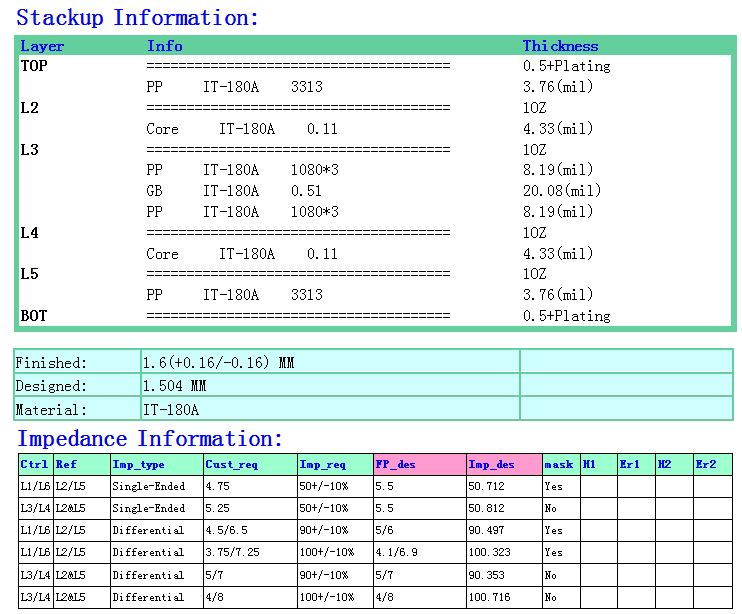
\includegraphics[angle=0,width=14cm]{images/LagenaufbauBB.jpg}
\caption{Lagenaufbau und Impedanzen des BBB}
\label{LagenaufbauBB}
\end{figure}


\section{Layout des PCB}

\subsection{Änderungen}
Am Layout des PCB, welches von der 'Element 14'-Homepage stammt, wurden folgende Änderungen vorgenommen:

%TODO detailierter; evt. Bilder
\begin{itemize}
\item Die Leiterbahnbreiten für die kontrollierten Impedanzen wurden entsprechend angepasst
\item Alle Änderungen für das Upgrade auf die Revision C (siehe \ref{sec:upgrade_rev_c}).
\item Der obere und unter Beschriftungsdruck wurde so angeordnet, dass die Designatoren gut sortiert und lesbar sind
\end{itemize}


\subsection{Kritische Stellen des Layouts}
Bei digitalen Hochgeschwindigkeitsübertragungen ist die Signalintegrität von grosser Bedeutung. Die Signalintegrität beschreibt, wie gut das gesendete Signal des Senders mit dem Signal übereinstimmt, welches der Empfänger am anderen Ende der Leitung empfängt. Wenn die Signalintegrität zu klein ist, kann es zu Datenverlusten führen. Dieser Datenverlust kann dazu führen, dass die Datenverbindung nicht mehr brauchbar ist. Wenn z.B. die Signalintegrität der Verbindung zwischen dem Prozessor und dem RAM zu schlecht ist, kann der Prozessor den RAM gar nicht mehr nutzen. Da der BBB ohne RAM nicht lauffähig ist, muss dies unbedingt verhindert werden.

Für eine gute Signalintegrität muss unter anderem die Impedanz der Leiterbahnen stimmen. Dieses Thema wurde bereits im Kapitel \ref{aufbauPCB} diskutiert. Zusätzlich müssen alle Leiterbahnen gleich lang sein, damit alle Signale gleichzeitig ankommen. Elektromagnetische Störungen von aussen können die Signalintegrität ebenfalls beeinflussen.

In Abbildung \ref{kritischeStellenBBB} sind alle Leiterbahnen, bei denen die Signalintegrität ein kritischer Faktor sein könnte, rot eingerahmt. Ohne detailliertes Wissen über digitale Signalintegrität, sollte das PCB Layout in diesem Bereich nicht geändert werden.

\begin{figure}[!ht]
\centering
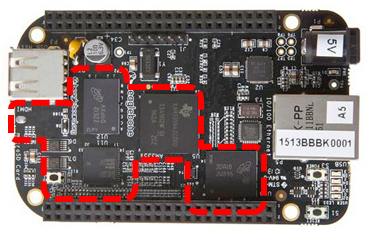
\includegraphics[angle=0,height=5cm]{images/BBB_kritische_stellen.png}
\caption{Kritische Stellen des BBB}
\label{kritischeStellenBBB}
\end{figure}




\section{Produktion der Prototypen}


\subsection{Vorgehen}
Die PCBs wurden von der Firma 'multi-cb' gefertigt. Die fertigen PCB sind dann beim Industriepartner Variosystems bestückt worden. Es wurden 10 PCBs bestellt, fünf davon sind bestückt worden.

Bei einer Bestückung durchläuft das PCB mehrere Stationen. Zuerst wird die Lötpaste auf das PCB aufgetragen. Anschliessend werden alle Bauteile durch einen Pick-and-Place-Roboter auf dem PCB platziert. In einem Reflow-Ofen wird dann das ganze PCB inklusive Bauteile und Lötpaste erhitzt, so dass die Bauteile endgültig mit dem PCB verlötet werden. Diese Schritte werden einmal für die Oberseite und einmal für die Unterseite ausgeführt. Mit einem Röntgengerät können dann auch die Lötstellen unter einem Bauteil kontrolliert werden.

Aufgrund von Firmenrichtlinen konnten bei der Bestückung leider keine Fotos von der Produktionsstrasse geschossen werden.


\subsection{Lötpaste}
Bei der ersten Station der Produktion wurde zuerst eine Lötpastenmaske aus dünnem Stahlblech genau über das PCB gelegt. Die Ausschnitte des Bleches entsprechen dem Layer \textit{Top Paste} und \textit{Bottom Paste} im PCB Dokument. Über diese Maske wurde feinkörnige, bleifreie Lötpaste gestrichen, die bei den Aussparungen der Maske auf dem PCB haften bleibt.

Der Nutzenrand des PCBs (siehe Abbildung XXX) war hier von grossem Vorteil. Dank diesem Rand konnte das PCB problemlos auf dem Förderband fixiert werden, ohne dass Lötstellen verdeckt werden. Nachdem die Lötpaste aufgetragen wurde, wurde das PCB auf einem Förderband zum Pick and Place Roboter transportiert.
%TODO Foto PC mit Nutzenrand


\subsection{Pick-and-Place-Roboter}
Im Pick-and-Place-Roboter wurden alle SMT Bauteile bestückt. Der Roboter platziert dabei alle SMT Bauteile auf dem PCB, durch die Lötpaste schwach auf dem PCB haften.

Das Einrichten der Maschine war ein sehr grosser Initialaufwand. Nachdem der Roboter aber richtig eingestellt wurde, ging das Bestücken zügig und ohne grössere Probleme voran. Aus diesem Grund ist diese Maschine nur bei grossen Stückzahlen effizient. 

Der Roboter hat leider immer wieder Bauteile verloren, die mühsam in der Maschine gesucht werden mussten. Da nicht alle Bauteile wieder gefunden werden konnten, musste eine HDMI-Schutzdiode (D6) und drei LEDs (D1, D2 und D3) nachbestellt und nachträglich von Hand aufgelötet werden.

Beim Bestücken wurde festgestellt, dass die Mini-USB Buchse (P4) nicht genau den richtigen Footprint hatte. Dieser war aber ähnlich genug, dass die Buchse trotzdem aufgelötet werden konnte. Der Footprint des $\mu$SD-Kartenhalters (P10) war ebenfalls fehlerhaft und konnte nicht aufgelötet werden. Diese Bauteile wurden anschliessend im eCAD Projekt mit den entsprechenden Bauteilen mit den richtigen Footprints ersetzt. Die $\mu$SD Kartenhalter wurden nachbestellt und von Hand eingelötet.


\subsection{Reflow Ofen}
Das bestückte PCB wurde auf dem Förderband durch den Reflow-Ofen geführt. Der Ofen hatte verschiedene Temperaturzonen, um eine optimale Lötung zu ermöglichen. Es wurde ein Standard-Temperaturprofil für 6-Lagige PCBs verwendet. Das verwendete Temperaturprofil findet sich im Anhang unter dem Kapitel \ref{sec:anhang_reflowofen_temeperaturprofil}.


\subsection{THT Bauteile}
Die THT Bauteile können nicht mit dem Roboter bestückt werden und müssen von Hand eingesteckt werden. Diese Bauteile können dann aber automatisiert mit einer Selektiv-Lötanlage gelötet werden. Im Rahmen dieser Arbeit wurden allerdings alle THT Bauteile der fünf Prototypen von Hand eingelötet.

Die Bohrungen für die beiden 46-Pin-Header waren zu klein. Es wurden 46-Pin-Header mit kleineren Pins nachbestellt und anschliessend von Hand bestückt und gelötet. Das eCAD Projekt wurde entsprechend ergänzt.


\subsection{Röntgengerät}
Viele Bauteile haben an der Unterseite Lötstellen, die von Auge unmöglich zu kontrollieren sind. Mit einem Röntgengerät liessen sich diese Stellen aber problemlos von allen Seiten durchleuchten. Dabei wurde neben der Position des Bauteils auch die Qualität der Lötstellen kontrolliert. Für ein ungeübtes Auge ist es allerdings kaum ersichtlich, ob eine Lötstelle gut oder schlecht ist. Der Operator vor Ort konnte dies aber in einem kurzen Augenblick feststellen. Das Bild in Abbildung \ref{fig:roentgenbildProzessor} wurde mit einem Röntgengerät gemacht und zeigt den Prozessor (U5) und den LAN-Chip (U14) im Hintergrund. Im Anhang XXX sind noch weitere Röntgenbilder angehängt.

%TODO Anhang Röntgenbilder

Zur Qualitätskontrolle wurde der erste Prototyp mit dem Röntgengerät durchleuchtet. Die Röntgenbilder zeigten, dass alle Lötstellen in Ordnung waren und die Bauteile alle richtig platziert wurden.

\begin{figure}[!ht]
\centering
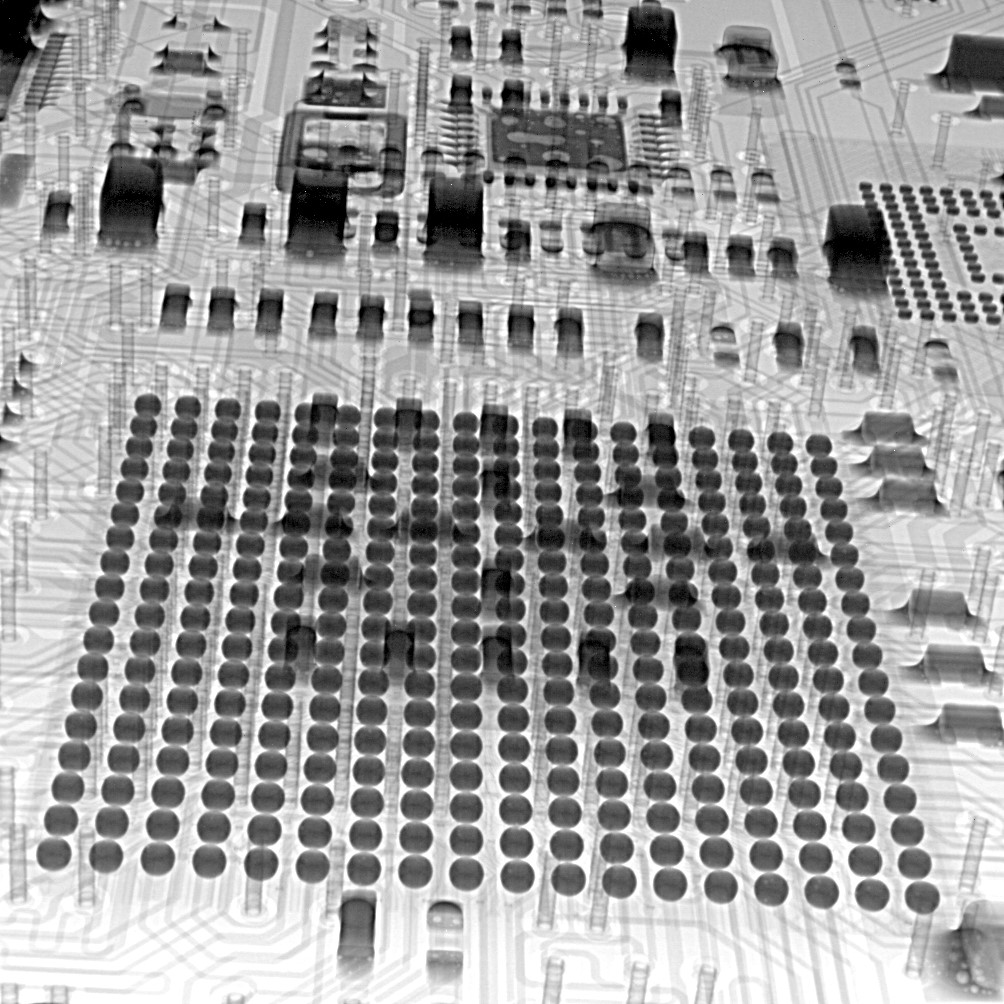
\includegraphics[angle=0,height=10cm]{images/Roentgenbild_U5_2.jpg}
\caption{Röntgenbild vom Prozessor}
\label{fig:roentgenbildProzessor}
\end{figure}



%	\chapter{ComCape}


\section{Übersicht}
Das ComCape, oder Communication Cape, ist eine zusätzliche Platine, welche sich auf den originalen BeagleBone Black oder auf das BeagleBone-Derivat stecken lässt. Ein Cape ist eine Platine, die eigens als Erweiterung für den BeagleBone entwickelt wurde. Solche Capes können den BBB zum Beispiel mit WLAN-Funktionalität erweitern und sind auch kommerziell erhältlich.

Das ComCape ist speziell für die Firma Variosystems entwickelt worden. Es erweitert den BBB, im Gegensatz zu den bereits erhältlichen Capes, um mehrere Funktionen:

\begin{itemize}
\item WLAN: Kabelloses Internet via Wireless LAN
\item GSM: Kabelloses Internet über das mobile Internet
\item BLE: Ermöglicht dem BBB eine drahtlose Verbindung über Bluetooth Low Energy
\item LCD: Über einen Flachbandstecker kann ein LCD mit kapazitivem Multi-Touch angeschlossen werden
\end{itemize}



\section{Allgemeiner Aufbau des ComCape}

\subsection{Elektrisches Schema}
Wie auch der BBB ist das ComCape auf 7 Top-Level Blätter verteilt:

\begin{itemize}
\item P01: Titelblatt
\item P02: WLAN 1/2
\item P03: WLAN 2/2
\item P04: GSM 1/2
\item P05: GSM 2/2
\item P06: BLE
\item P07: Stiftleiste und LCD-Stecker
\end{itemize}

Im Folgenden wird nur noch auf die Seitennummer des Schema (P01...P07) verwiesen, und nicht mehr auf den Namen.

Für alle nicht benutzten Pins der Bauteile wurden Testpunkte hinzugefügt, damit diese auch nachträglich noch zugänglich sind.

Alle Signale, die zum BBB führen, sind über einen 0$\Omega$ Widerstand geführt. So können alle Bauteile elektrisch vom BBB getrennt werden. Dies kann besonders nützlich sein, wenn ein Teil des ComCapes getrennt von dem Rest getestet werden will.

%Alle Designatoren von P02 starten mit 1, die von P03 mit 50, die Designatoren von P04 mit 100 u
%TODO Designatoren beschreiben

\section{Layout PCB}
Das PCB ist in drei Teile aufgeteilt. Auf dem unteren Teil befinden sich ausschliesslich Bauteile für das GSM, während der Mittlere Teil für WLAN-Bauteile reserviert ist. Im oberen Teil befinden sich neben dem Stecker für den LCD auch noch die Komponenten für das Bluetooth Modul.

Das Bluetooth-, das WLAN- und das GSM-Modul haben auch auf der Unterseite des ChipgehäuseS Pins, die gelötet werden müssen. Es ist nicht möglich, diese Bauteile von Hand zu löten. Aus diesem Grund wurden alle Bauteile auf der oberen Seite des PCBs im Reflow-Ofen gelötet. Für den Prototypenbau wurden die Bauteile auf der unteren Seite von Hand gelötet. Beim Erstellen des PCB-Layouts wurde darauf geachtet, dass möglichst viele Bauteile auf der oberen Seite platziert wurden. Zusätzlich wurde darauf geachtet, dass die linearen Spannungsregler, welche viel Abwärme produzieren, für die bessere Wärmeabgabe ebenfalls auf der oberen Seite platziert wurden. Die drei Module befinden sich ebenfalls auf der oberen Seite des PCBs.


\subsection{Grösse und Form des PCB}
Das ComCape sollte nicht grösser sein, als das LCD. Wenn man das LCD im Hochformat über das ComCape legt, ist das Cape aus diesem Grund gleich breit wie das LCD. Oben und unten wurde das Cape um je 1cm verlängert, um noch Befestigungsbohrungen platzieren zu können.

Da beim BBB die Ethernet-Buchse sehr hoch ist, hat das Cape auf der linken Seite eine Aussparung für diese Buchse. Zusätzlich ist die obere Hälfte des ComCapes schmaler, damit die Taster S1 und S3 vom BBB besser zugänglich sind. Anhang \ref{sec:anhang_befestigungsbohrungen} zeigt den Umriss des ComCapes und die Vermassung der Befestigungsbohrungen.



\section{Wirless LAN}
Für das Wireless LAN wurde das WL1835 Modul von Texas Instruments verwendet.

Für den BBB existiert bereits ein WLAN-Cape, welches gekauft werden kann. Auf diesem Cape ist ein WL1835 Modul verbaut. Das elektrische Schema und die Gerberdaten von diesem Cape sind frei erhältlich\cite{boardZooWLANCape}. Aus diesen Gründen haben wir das 'WL1835MOD W/ Chip Antenna' Cape als Referenzdesign verwendet.

%TODO Bild WLAN Cape


\subsection{Stromversorgung}
Die VDD\_3V3B Spannungsversorgung vom BBB wird für die prozessorseitige Spannungsversorgung des Spannungspegelwandlers verwendet.

Für die 3.3V-Spannungsversorgung wurde der gleiche lineare Spannungsregler verwendet, wie im Referenzdesign. Dieser Regler kann bis zu 1.5A liefern. Der effektive Strombedarf des Moduls ist abhängig vom Betriebsmodus und lässt sich nur schwer einschätzen. Deshalb wurde derselbe, vermutlich überdimensionierte, Spannungsregler wie im Referenzdesign verwendet. Der effektive Dauer- und Spitzen- Strom lässt sich im Betrieb mit einem Messwiderstand und einem Oszilloskop über dem Steckkontakt 'X1' messen.

Die 1.8V-Spannungsversorgung wird nur für die digitale Kommunikation verwendet. Aus diesem Grund wurde der 0.4A-Spannungsregler, welcher im Referenzdesign verwendet wird, mit einem 0.15A-Spannungsregler ersetzt, der auch in der Standardbibliothek von Variosystems zu finden ist. Auch bei dieser Versorgung lässt sich der effektive Strombedarf über den Steckkontakt 'X2' messen.

\subsection{Antenne}
Das ComCape unterstützt von der Hardware her zwei Antennen. In der Software wird aber nur eine unterstützt. Mehr dazu im Kapitel \ref{sec:wlan_varianten} weiter unten.

Bei der Antenne 1, welche gleichzeitig für WLAN und Bluetooth (ist in der Software nicht implementiert) genutzt wird, kann entweder die Kombination aus Chip- und PCB- Antenne oder eine externe Antenne verwendet werden. Wenn die externe Antenne verwendet werden soll, muss C54 eingelötet sein. Soll die PCB Antenne verwendet werden, muss C54 wieder ausgelötet und stattdessen C55 eingelötet werden.

Die externe Antenne kann über eine U.FL-Buchse angeschlossen werden.

Das PCB-Layout für die Chipantenne wurde aus dem Datenblatt der Chipantenne kopiert.

Für die Verbindung zwischen dem Modul und den Antennen wird eine Übertragungsleitung mit einer Wellenimpedanz vom 50$\Omega$ benötigt. Im Hardware User Guide von Telit[XXX] wird eine Übertragungsleitung mit den Massen, wie in Abbildung \ref{50OhmTransmissionLine} empfohlen. Berechnungen mit der Software 'txLine' haben gezeigt, dass sich die Wellenimpedanz nicht signifikant ändert, wenn diverse Masse, wie zum Beispiel die Dicke des PCB oder die Dielektrizitätskonstante des Dielektrikums, sich um 10\% ändern. Aus diesem Grund kann bei der Herstellung des PCB auf eine kontrollierte Impedanz verzichtet werden.

%TODO Quelle HW userguide Telit
%TODO Berechnungen

\begin{figure}[!ht]
\centering
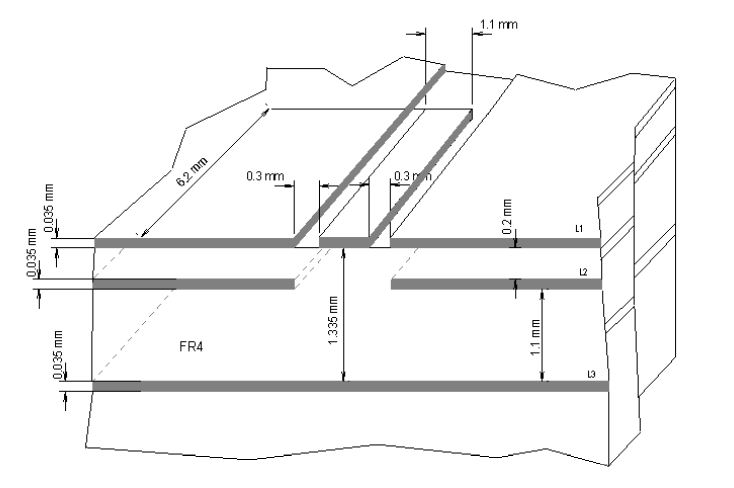
\includegraphics[angle=0,height=8cm]{images/50OhmTransmissionLine.jpg}
\caption{50$\Omega$ Übertragungsleitung}
\label{50OhmTransmissionLine}
\end{figure}


\subsection{32kHz Taktsignal}
Das Modul benötigt einen 32,768kHz Takt. Je nachdem, welche Widerstände eingelötet werden, können verschiedene Quellen für den Takt ausgewählt werden. Da bei der Planung des Capes nicht klar war, welche der Varianten funktionieren würde, sind alle drei Varianten auf dem Cape verwirklicht.

\textbf{R32: Lokaler Oszillator}: Der Oszillator erzeugt auf dem Cape einen 32kHz Takt und wird sonst nirgends verwendet. Dies ist die Standardvariante, da sie auch im Referenzdesign verwendet wird, und am wahrscheinlichsten funktioniert. Allerdings ist dieser Oszillator relativ teuer.

\textbf{R24: Von BBB erzeugt, mit Pegelwandler}: Diese Variante nutzt das Taktsignal, welches vom BBB erzeugt wird. Das 3.3V Signal wird dann mit einem TXS0108E auf 1.8V gewandelt. Ungünstiger weise wird dafür extra ein separater Pegelwandler benötigt.

\textbf{R28: Von BBB erzeugt, mit Spannungsteiler}: Auch diese Variante nutzt den Takt, der vom VBB erzeugt wird. Der Spannungspegel wird diesmal aber mit einem einfachen Spannungsteiler aus zwei Widerständen auf 1.8V gebracht. Das WLAN-Modul hat beim Eingang für dieses Taktsignal einen Eingangswiderstand von 1M$\Omega$\footnote{Quelle: Datenblatt WL1835MOD Seite 11}[XXX] und kann deshalb für diese Berechnung vernachlässigt werden. Wenn diese Variante funktioniert, ist sie am günstigsten und den anderen beiden vorzuziehen.
$$U_{out} =  3.3V * \dfrac{R29}{R29+R27} = 3.3V * \dfrac{4.7k\Omega}{4.7k\Omega+3.9k\Omega} = 1.80V$$

%TODO Quelle [XXX]

\subsection{Digitale Verbindung zum Prozessor}
Die WLAN-Daten werden über eienen SDIO Bus zum Prozessor übertragen. Der Spannungspegel wird dabei mit zwei TXS0108E Spannungswandlern von den 1.8V des Moduls auf 3.3V für den Prozessor gewandelt. Dieser Wandler funktioniert auf beide Richtungen, so dass auch Signale vom Prozessor zum WLAN-Modul auf den richtigen Pegel gewandelt werden.

Auf den zweiten TXS0108E kann verzichtet werden, wenn das 32kHz Taktsignal nicht vom VBB erzeugt wird.

\subsection{Varianten}\label{sec:wlan_varianten}
Das WL1835 Modul unterstützt neben einem Design mit zwei Antennen auch noch Bluetooth. Im ComCape wird Bluetooth und die zweite Antenne aber von der Software nicht unterstützt. Von der Hardware ist aber alles Nötige vorhanden. Die zweite Antenne könnte für MIMO oder eine MRC Konfiguration genutzt werden. MIMO steht für 'Multiple Input Multiple Output', damit kann im Vergleich zu einem Design mit einer Antenne (SISO = Single Input Single Output) die Bandbreite erhöht werden. Mit MRC oder 'Maximum Ratio Combining' kann die Reichweite des Signals erhöht werden.

Es existieren zum WL1835 pinkompatible Module, welche ein Design mit zwei Antennen, Bluetooth oder beides nicht unterstützen. In der Tabelle \ref{tab:wlanVarianten} sind alle vier Module und deren Funktionen aufgelistet.

\begin{table}

    \begin{tabular}{ | c | c | c | c | c |}
    \hline
    \textbf{Modul}		& \textbf{2.4-GHZ SISO}	& \textbf{2.4-GHZ MIMO}	& \textbf{2.4-GHZ MRC}	& \textbf{Bluetooth} \\ \hline
    
     WL1835MOD	& X				& X	 			& X				& X \\ \hline    
    
     WL1831MOD	& X				&	 			& 				& X \\ \hline  
    
     WL1805MOD	& X				& X	 			& X				&  \\ \hline  
    
     WL1801MOD	& X				& 	 			& 				&  \\ \hline  
    
    
    \end{tabular}
\caption{Varianten des WLAN Moduls}
\label{tab:wlanVarianten}
\end{table}


%TODO WAS NICHT FUNKTIONIERT UND WARUM


\section{GSM}


\subsection{Stromversorgung}
	
%	
%	\glossary{name={eCAD},description={Electronic Computer-Aided Design: Computerprogramm zum Entwerfen von elektrischen Layouts und PCB}}

\glossary{name={PCB},description={Printed Circuit Board: Elektronische Platine, auf welcher die elektronischen Bauteile aufgelötet werden. Wird auch Platine genannt.}}

\glossary{name={BBB},description={BeagleBone Black: Kostengünstiger Einplatinen-Computer von Texas Instruments}}

\glossary{name={BBB-Derivat},description={BeagleBone-Derivat: Das Produkt, das in dieser Bachelorarbeit in Zusammenarbeit mit Variosystems hergestellt wurde. Es hat den selben Funktionsumfang wie der BBB}}

\glossary{name={BeagleBone Black},description={Siehe BBB}}

\glossary{name={PHY},description={PHYsical Layer: Spezieller integrierter Schaltkreis der die modulierten analogen Daten des LAN-Anschlusses in digitale Daten wandelt und umgekehrt. Dieses Bauteil wird zusammen mit einer RJ45-Buchse und einem MAC für eine Ethernet-Schnittstelle benötigt}}

\glossary{name={MAC},description={Media Access Control: Dieser Controller wird zusammen mit einer RJ45-Buchse und einem PHY für eine Ethernet-Schnittstelle benötigt }}

\glossary{name={HDMI},description={High Definition Multimedia Interface: Eine Schnittstelle für die volldigitale Übertragung von Audio- und Videodaten}}

\glossary{name={eMMC},description={Embedded Multimedia Card: Massenspeicher mit Flashspeicher, MMC-Interface und Controller. Ersetzt im BBB die Festplatte}}

\glossary{name={awk},description={Skriptsprache zur Bearbeitung und Auswertung strukturierter Textdaten, beispielsweise CSV-Dateien}}

\glossary{name={Designator},description={Eindeutige Bezeichnung aus einem Buchstaben und einer Zahl für ein elektrisches Bauteil in einem Schema oder PCB-Layout}}

\glossary{name={Cape},description={Erweiterung speziell für den BBB}}

\glossary{name={WLAN},description={Kabelloser Standard für LAN}}

\glossary{name={BLE},description={Bluetooth Low Energy: Standard für eine Funktechnik, die mit sehr geringen Stromverbrauch Geräte in einer Umgebung von 10 Meter vernetzen kann}}

\glossary{name={LCD},description={Liquid Cristal Display: Flachbildschirm}}

\glossary{name={SDIO},description={Secure Digital Input Output: Vielseitiger Datenbus, welcher unter Anderem für SD-Karten verwendet wird}}

\glossary{name={I$^2$C},description={Inter-Integrated Circuit: serieller Datenbus, welcher für die Kommunikation zwischen Bauteilen auf einem PCB verwendet wird}}

\glossary{name={EEPROM},description={Electrically Erasable Programmable Read-Only Memory: nichtflüchtiger, elektronischer Speicher für kleine Datenmengen}}

\glossary{name={RAM},description={Random-Access Memory: wird von Prozessoren als Arbeitsspeicher benötigt}}

\glossary{name={Python},description={Universelle Programmiersprache}}

\glossary{name={SMT},description={Surface Mounted Technology: Oberflächenmontage. Die elektrischen Bauteile werden nur auf der Oberfläche des PCB gelötet}}

\glossary{name={THT},description={Through Hole Technology: Durchsteckmontage. Die Bauelemente haben Drähte als Anschluss, die durch das PCB gesteckt werden}}

\glossary{name={McASP},description={Multichannel Audio Serial Port: Datenbus für Audiodaten}}

\glossary{name={Footprint},description={Die Umrisse von Lötflächen von elektrischen Bauelementen auf einer Leiterplatte}}





\glossary{name={USB},description={Universal Serial Bus: Serielles Bussystem zur Verbindung eines Computers mit externen Geräten}}

\glossary{name={LAN},description={Local Area Network: Netzwerk mit einer Ausdehnung, von i.d.R. mehreren Räumen}}

\glossary{name={SPI},description={Serial Peripheral Interface: Bus-System nach dem Master-Slave-Prinzip zur Verbindung von digitalen Schaltungen}}

\glossary{name={GPIO},description={General Purpose Input/Output: Schnittstelle die die meisten Mikrocontroller besitzen um mit externen Geräten zu kommunizieren}}

\glossary{name={RS232},description={Standard für eine serielle Schnittstelle mit definiertem Spannungspegel}}

\glossary{name={UART},description={Standard für eine serielle Schnittstelle}}





\renewcommand{\glossaryname}{Glossar}
\printglossary

	\begin{thebibliography}{BA}
%	\bibitem[VAR-15]{variosystems} \emph{Homepage; Variosystems}
%	\\http://www.variosystems.com/index.php/de/ueber-uns
%	\\Stand vom 23.07.2015

	\bibitem[ELI-15]{bbbOrcad} \emph{Homepage: Embedded Linux Wiki}
	\\http://elinux.org/Beagleboard:BeagleBoneBlack\#LATEST\_PRODUCTION\_FILES\_.28C.29
	\\Stand vom 05.01.2015
	
	\bibitem[ELE-15]{element14AltiumBBB} \emph{Homepage: Element 14}
	\\www.element14.com/community/docs/DOC-54121?ICID=beagleboneblack-space\#downloads
	\\Stand vom 05.01.2015
	
	\bibitem[ADA-15]{adafruitSRM} \emph{Homepage: Adafruit}
	\\www.adafruit.com/datasheets/BBB\_SRM.pdf
	\\Stand vom 31.07.2015
	
	\bibitem[BOA-15]{boardZooWLANCape} \emph{Homepage: Board Zoo}
	\\http://boardzoo.com/index.php/beaglebone/beaglebone-wl1835mod-w-chip-antenna.html\#.VbugbMDtlBc
	\\Stand vom 31.07.2015
	



%\cite{adafruitSRM} 

\end{thebibliography}








	\appendix
	\setcounter{page}{1}
	\renewcommand{\thepage}{\Alph{section} \arabic{page}}
	\addchap*{\appendixname}

	\newenvironment{nosectionintoc}{
		\setcounter{secnumdepth}{3}
		\addtocontents{toc}{\protect\setcounter{tocdepth}{0}\ignorespaces}
	}
	{\setcounter{secnumdepth}{3}%
	\addtocontents{toc}{\protect\setcounter{tocdepth}{3}\ignorespaces}}

	\begin{nosectionintoc}	%taucht nicht im Inhaltsverzeichnis auf
		\makeatletter
		\@addtoreset{figure}{section}
		\@addtoreset{table}{section}
		\makeatother
	    \renewcommand{\thefigure}{\Alph{section}.\arabic{figure}}
	    \renewcommand{\thetable}{\Alph{section}.\arabic{table}}
    	\renewcommand{\thesection}{\Alph{section}}
	    \let\oldsection=\section
	    \def\resetpage{\setcounter{page}{1}}
	    \renewcommand{\section}[1]{\oldsection{#1}\resetpage}

%		\clearpage
\section{Fachmodulbericht}\label{sec:anhang_main}

\includepdf[pages=-,angle=0,scale=0.8,frame]{anhang/fachmodulbericht/Dokumentation_Fachmodul.pdf}
%\includepdf[pages={1-2},angle=90,scale=0.8]{anhang/Dokumentation_Fachmodul.pdf}

%\newpage
%\section{Pflichtenheft}\label{sec:anhang_pflichtenheft}
%\includepdf[pages={1-9},scale=0.8,frame]{anhang/sonstiges/pflichtenheft.pdf}

\newpage

		\clearpage
\section{Test Case 8}\label{sec:anhang_test_case_8}

\begin{center}
  \makebox[\textwidth]{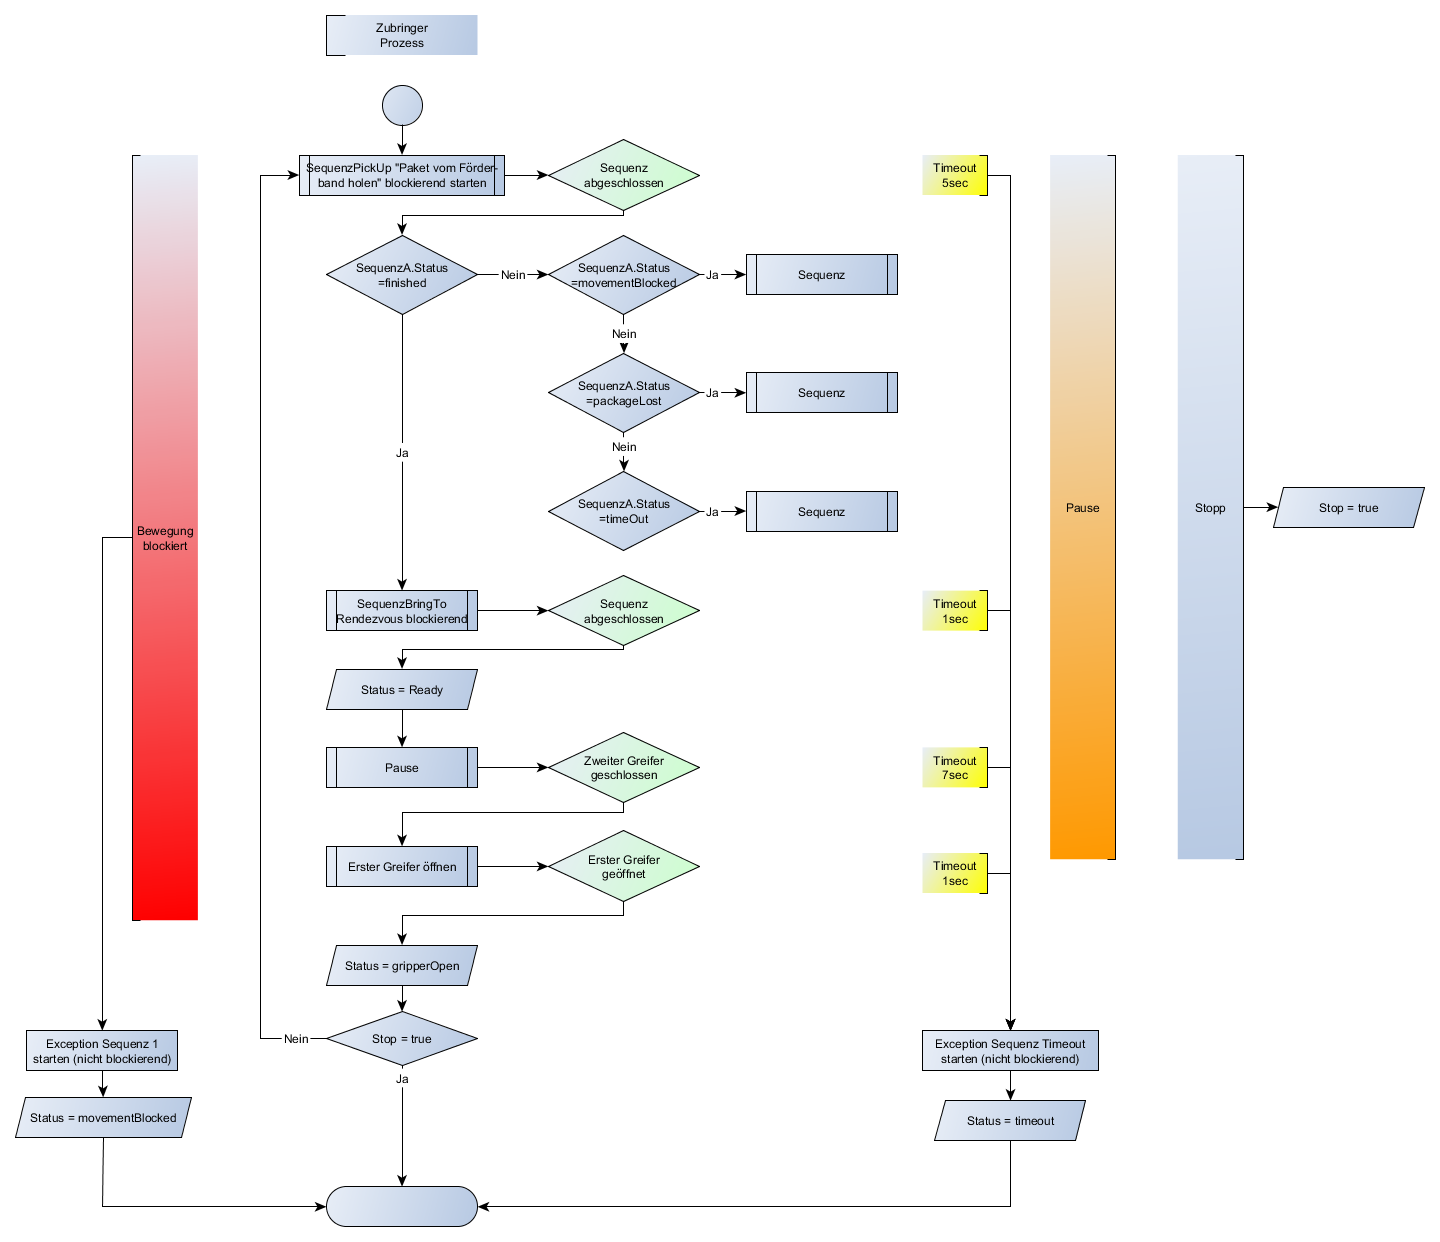
\includegraphics[width=\textwidth]{images/TestCase8Sequence1.png}}
%  \caption{Signalverlauf bei einem prellenden Schalter}
  \label{TestCase8Sequence1Picture}
\end{center}

\begin{center}
  \makebox[\textwidth]{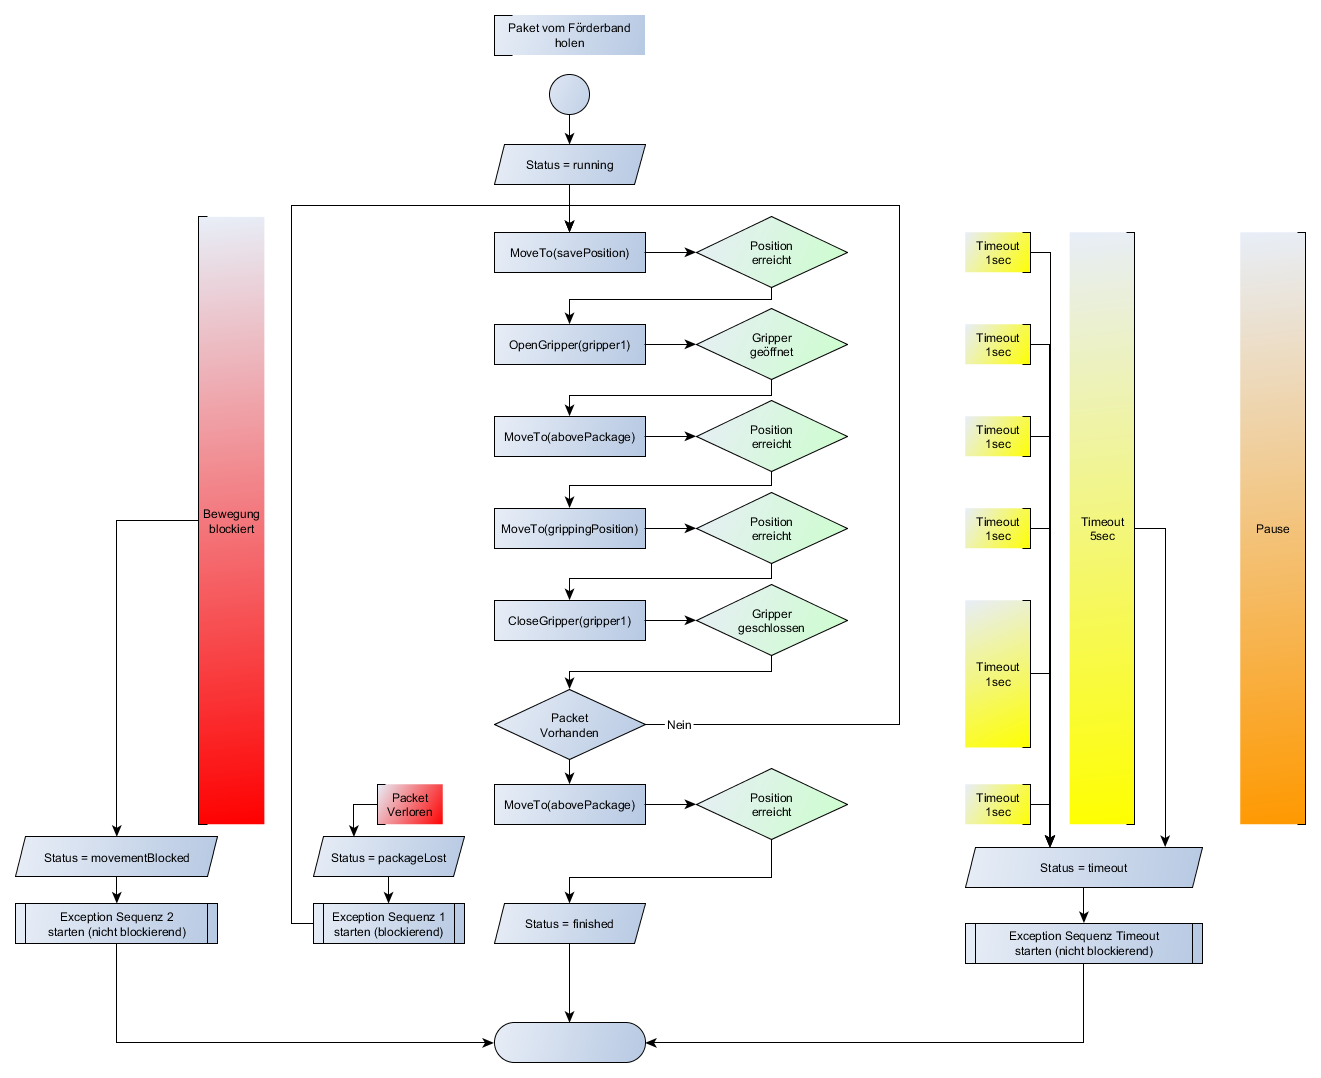
\includegraphics[width=\textwidth]{images/TestCase8Sequence2.png}}
%  \caption{Signalverlauf bei einem prellenden Schalter}
  \label{TestCase8Sequence2Picture}
\end{center}



%\subsection{Skizze Befestigungsbohrungen}\label{sec:anhang_befestigungsbohrungen}
%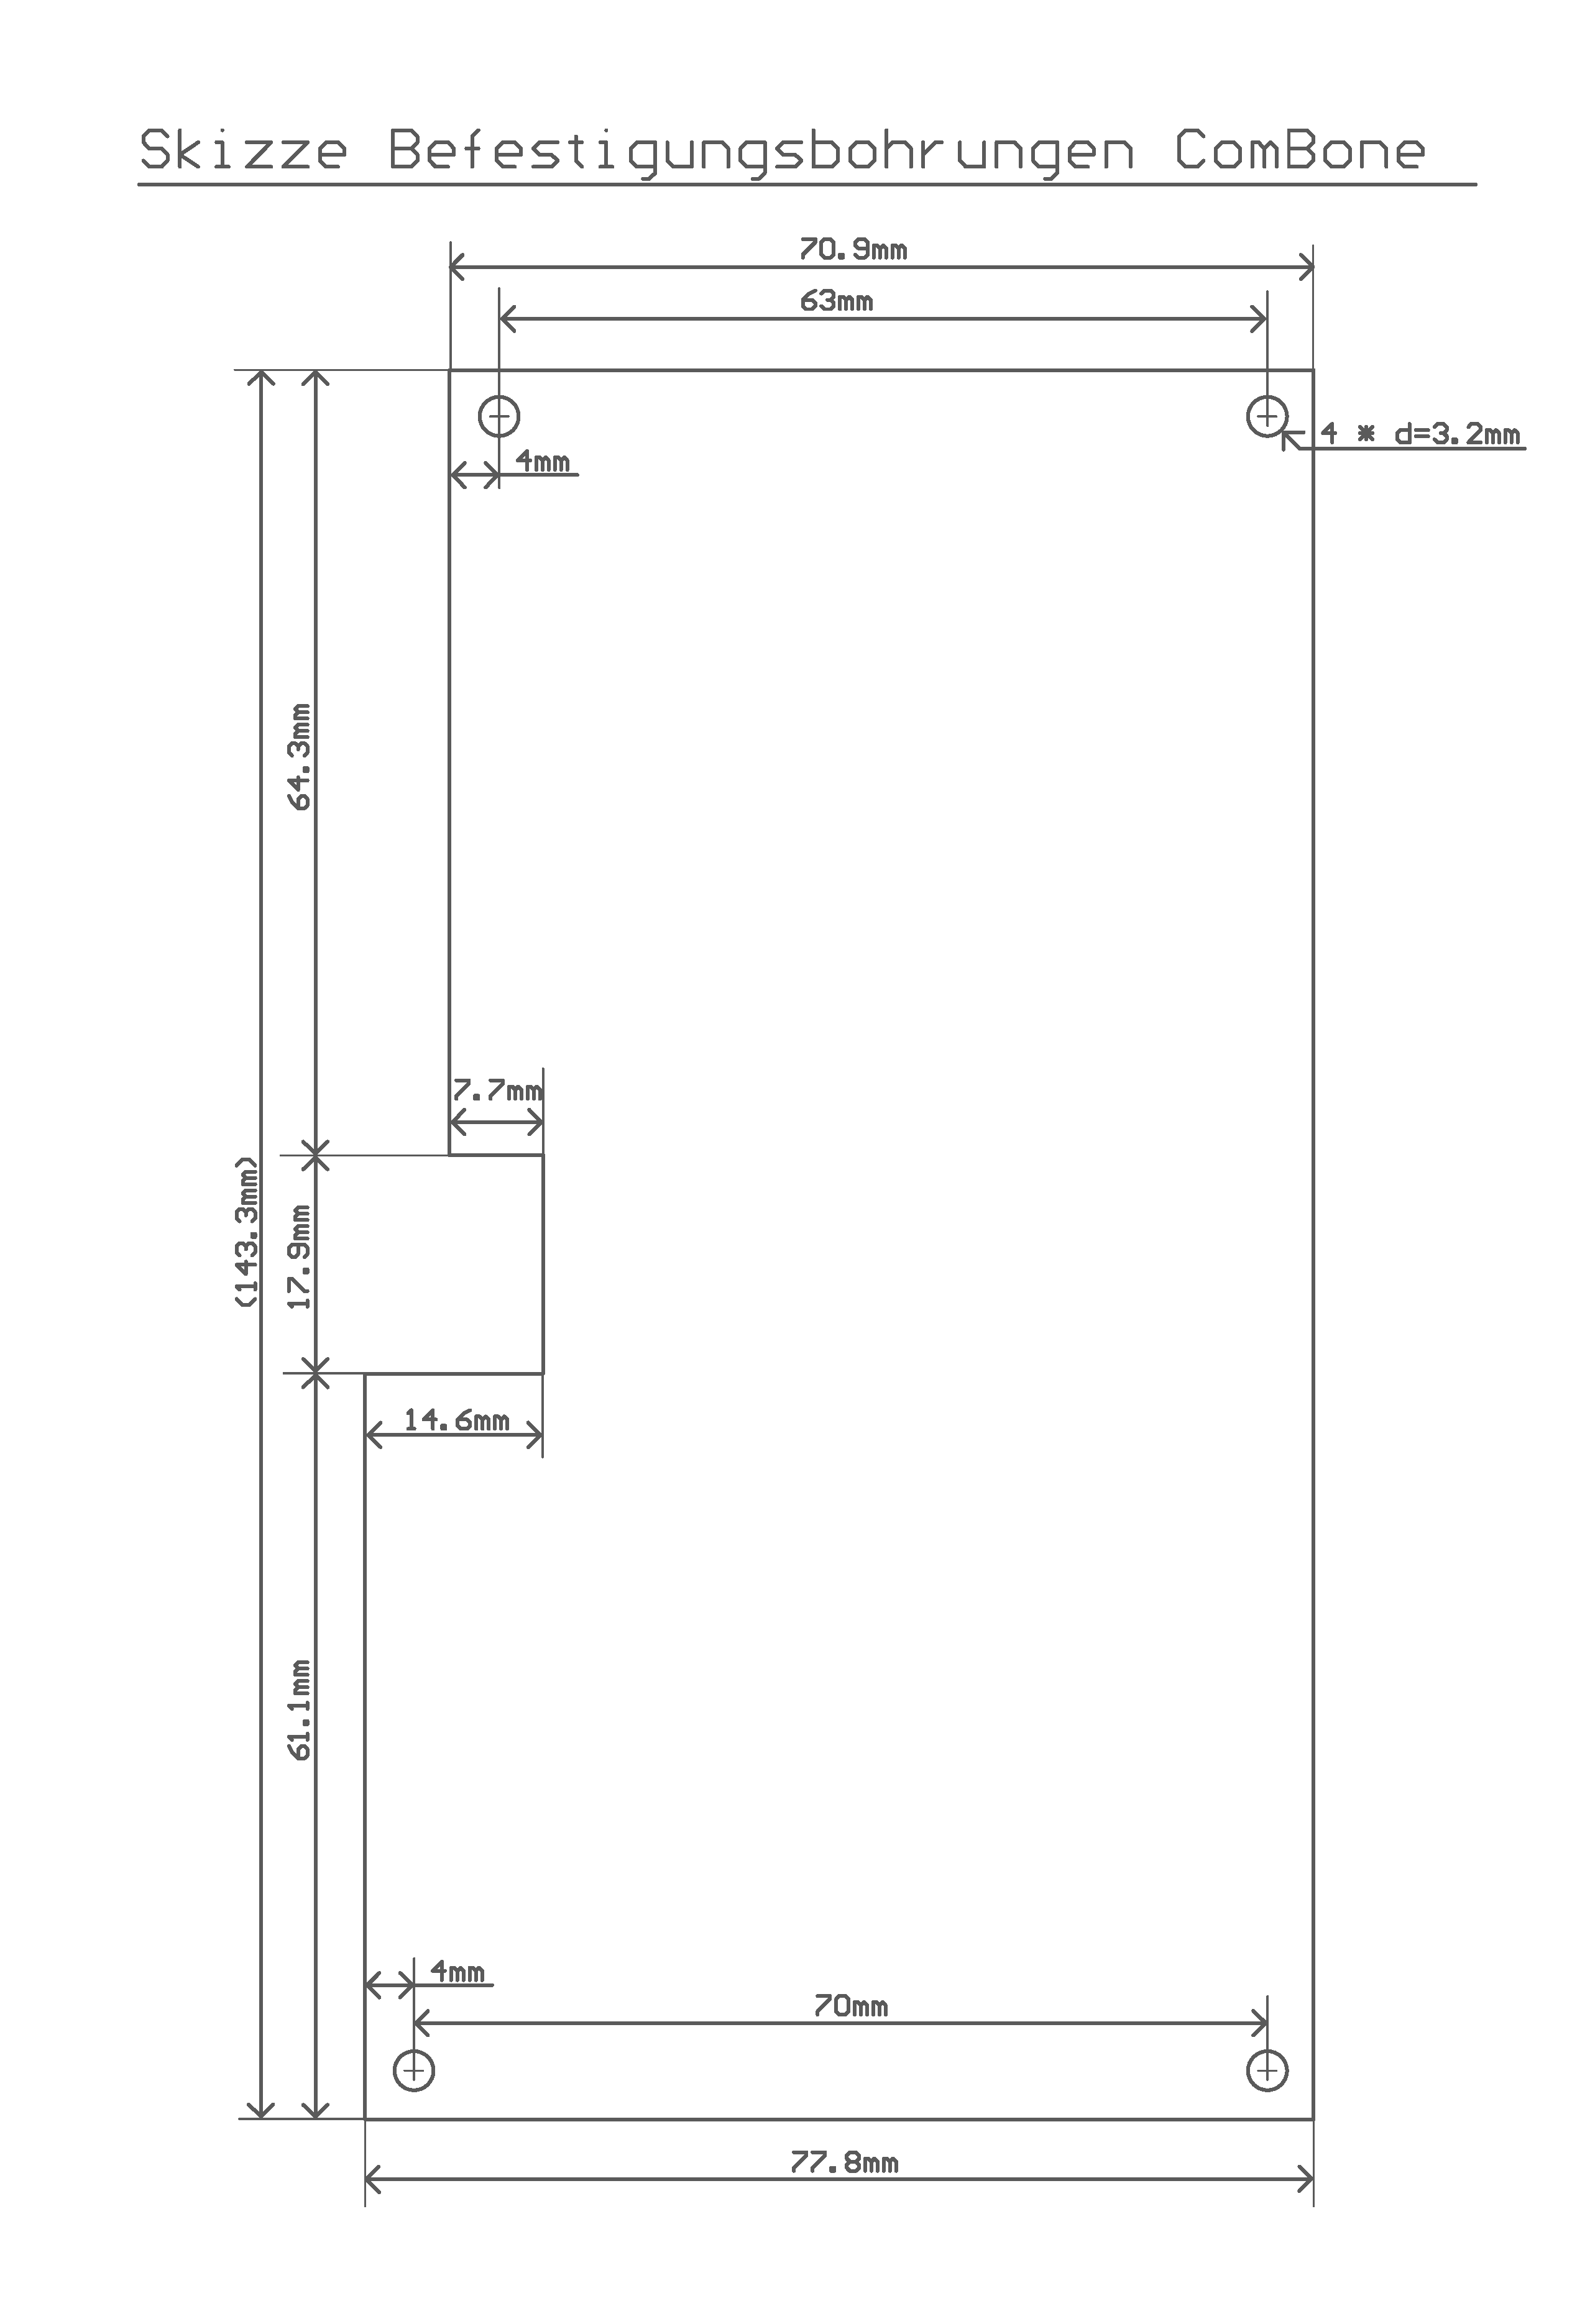
\includepdf[pages=-,pagecommand={\thispagestyle{scrheadings}},angle=0,scale=0.8,frame]{anhang/Elektronik/Skizze_Befestigungsbohrung_ComCape.PDF}




		
		
%
	\end{nosectionintoc}

\end{document}
